\chapter{Results and Discussion}\label{ch:5}

All figures in this chapter are computed out of fold under the leave-one-campaign-out protocol of Section 4.9 unless stated otherwise, from features lagged as described in Section 4.6.


\section{The alignment audit and what it costs}
\label{sec:5_1}

The first result of this chapter is not a prediction score. It is a property of the measurement export that determines what any prediction score on this data means.

The audit is simple. For each handover command at time tau, take the export row whose second contains tau --- that is, the row stamped at floor(tau), strictly before the command --- and ask whether its serving-cell identity is already the target of that command. If the row summarises the second before its timestamp, the answer should be no more often than chance.


\begin{table}[htbp]
\centering
\caption{The alignment audit: share of handovers whose target cell already serves in export rows around the command.}
\label{tab:5_1}
\vspace{0.4em}
\singlespacing
\footnotesize
\resizebox{\linewidth}{!}{%
\begin{tabular}{l c c c c c c}
\toprule
\textbf{Handovers considered} & \textbf{n} & \textbf{row t-3} & \textbf{row t-2} & \textbf{row t-1} & \textbf{row t+0} & \textbf{row t+1} \\
\midrule
all handovers & 938 & 23.7 \% & 21.7 \% & 15.6 \% & 75.9 \% & 86.2 \% \\
isolated (previous > 8 s earlier) & 291 & 12.1 \% & 12.1 \% & 11.7 \% & 74.6 \% & 89.7 \% \\
\bottomrule
\end{tabular}%
}
\end{table}

Table~\ref{tab:5_1} also bears on whether the one-row lag leaves residual contamination, and it shows none. Leakage from the aggregation rule would appear as a step at the last row before the command. Instead, the share of rows already showing the target cell falls from row $t-3$ to row $t-1$ in both subsets: from 23.7\% to 15.6\% across all handovers, and from 12.1\% to 11.7\% on isolated ones. It then jumps only at row $t+0$. The higher pooled level is a baseline effect rather than a lag effect: with 26.3\% of commands being ping-pong returns within 15~s and a median inter-command gap of 3.7~s, the next target cell has often served within the last few seconds. The model-side check points the same way. On quiet rows (no command in the previous 10~s), whose 238 positives all precede a command with no other command in the preceding 10~s, LightGBM reaches AUPRC 0.133 against a 4.3\% floor (3.1$\times$ lift, AUROC 0.772). On in-burst rows it reaches 0.212 against 11.2\% (1.9$\times$, AUROC 0.720) (Section~\ref{sec:5_8}, Table~\ref{tab:5_11}). The ordering holds for burst cutoffs from 5 to 20~s (Table~\ref{tab:A_5}). If residual burst contamination were carrying the result, lift would be highest inside bursts. It is lowest there, which is inconsistent with residual leakage driving the pooled 0.179.


\begin{table}[htbp]
\centering
\caption{What the one-row lag costs, with everything else held fixed.}
\label{tab:5_2}
\vspace{0.4em}
\singlespacing
\footnotesize
\resizebox{\linewidth}{!}{%
\begin{tabular}{l c c c c}
\toprule
\textbf{Feature alignment} & \textbf{AUPRC 1 s} & \textbf{AUROC 1 s} & \textbf{AUPRC 5 s} & \textbf{Dwell feature AUROC 1 s} \\
\midrule
Export row stamped t used at t (v1) & 0.600 & 0.911 & 0.560 & 0.873 \\
Export row lagged one sample (this work) & 0.179 & 0.777 & 0.475 & 0.664 \\
Change & -70 \% & -0.134 & -15 \% & -0.209 \\
\bottomrule
\end{tabular}%
}
\end{table}


\begin{table}[htbp]
\centering
\caption{Where the leak actually lives. One common row set of usable rows, identical folds, seeds and learner; only the set of columns shifted by one row changes. The serving-cell radio scalars are measured on whichever cell the export treats as serving, so after the end-of-second flip they describe the target rather than the source.}
\label{tab:5_2b}
\vspace{0.4em}
\singlespacing
\footnotesize
\resizebox{\linewidth}{!}{%
\begin{tabular}{l c c c c}
\toprule
\textbf{What is lagged by one row} & \textbf{Columns} & \textbf{AUPRC 1 s} & \textbf{AUROC 1 s} & \textbf{AUPRC 5 s} \\
\midrule
nothing (v1 alignment) & 0 & 0.607 & 0.911 & 0.558 \\
neighbour and gap columns only & 31 & 0.595 & 0.905 & 0.550 \\
serving-cell radio scalars only & 56 & 0.178 & 0.768 & 0.451 \\
every serving-relative column (GPS left at row t) & 92 & 0.159 & 0.748 & 0.439 \\
every export column (v2, as reported throughout) & 109 & 0.160 & 0.750 & 0.445 \\
control: Event A3 rule, same arms & - & 0.116 to 0.117 & - & - \\
\bottomrule
\end{tabular}%
}
\end{table}

The consequence for prediction is immediate. A model asked at time t for the probability of a handover in (t, t + 1] and given the row stamped t is being shown, most of the time, the answer. Table~\ref{tab:5_2} quantifies it on the same model, the same folds and the same features: the one-second AUPRC falls from 0.600 to 0.179 and AUROC from 0.911 to 0.777 when every export feature is lagged one row. At five seconds, where one second of misalignment matters less, the same change costs 0.560 to 0.475. The single-feature effect is starker: serving dwell time computed from the export's serving-cell column reaches AUROC 0.873 on its own, and the same quantity computed from signalling timestamps reaches 0.664.

Three points are worth stating plainly. First, this is not a defect of the instrument in the sense of a fault: a one-hertz export has to summarise a second, and a row that carries the state at the end of its second is a defensible choice. It is a defect of any analysis that assumes the opposite without checking. Second, the error is invisible to every check that does not involve the event clock --- the features are causal in appearance, no future label is used, and grouped splitting does not remove it, because the leak is inside the row rather than between rows. In the taxonomy of Kaufman et al. \cite{ref36} it is leakage in training examples rather than leakage in feature construction: no illegitimate feature was built, and no future row was consulted; the legitimate feature simply describes an interval that already contains the event. That class is the one their paper identifies as hardest to catch, because every syntactic check passes. Third, it is cheap to detect, and the audit above is the recommendation this thesis makes to anyone building a predictor on a drive-test export.

Why the row behaves this way is not a mystery, and stating the reason turns the observation into a prediction that can be falsified. A handover command is issued at an arbitrary instant $\tau$ inside the second $[t, t+1)$. Write $\delta = \tau - \lfloor\tau\rfloor$ for where inside the second the command falls, $x$ for the empirical diagnostic timestamp interval between the command arrival (\texttt{RRCConnection\-Reconfiguration}) and UE completion (\texttt{RRCConnection\-Reconfiguration\-Complete}), and


\begin{equation}\label{eq:5_1} m = 1 - \delta - x, \quad \text{with } \delta, x \text{ and } m \text{ all in seconds} \end{equation}

for the margin by which that change beats the close of the second. Crucially, $x$ represents an empirical protocol proxy derived from diagnostic completion timestamps in the decoded baseband log; it should not be conflated with the modem's internal serving-cell register commit, nor with the physical user-plane interruption time (which 3GPP TS~36.133 defines across physical-layer synchronisation and which diagnostic drive-test traces cannot independently establish). Baseband logging and export queuing latency inherently bounds the precision of this proxy. If the exporter writes one row per second carrying the state as of the end of the second, the row stamped $t$ shows the target cell when $m > 0$ and the source cell when $m < 0$. Nothing about the network enters: the defect is what end-of-second aggregation does to an event whose execution is two orders of magnitude faster than the grid.

On our own captures, decoded signalling records protocol completion timestamps for each handover (65\% of commands record a non-zero diagnostic completion interval; the ninetieth percentile is 99~ms and the largest is 105~ms). An in-sample diagnostic check on the 15 handovers whose diagnostic completion interval crosses the second boundary ($m < 0$) confirms zero contamination on the row stamped before the command (0/15; 95\% Wilson score interval [0.0\%, 20.4\%]). While the small sample size leaves up to 20.4\% contamination possible under chance, the mechanism is independently and conclusively verified across instruments on the 4,712-handover NUWiNS corpus below. Of the 923 handovers with $m > 0$, the row shows the target cell 77.1\% of the time. The same gradient appears in $\delta$ directly: on handovers isolated from any other by two seconds, contamination runs at 86.1\% for commands in the first quarter of the second and falls to 67.0\% for commands in the last quarter, where the margin is smallest. Panels (d) and (e) of Figure~5.1 show both.

The residual matters for honesty about the size of the effect. In 22.5\% of handovers the margin is positive and the row stamped t nevertheless shows the source cell; in 84\% of those the row stamped t+1 carries the target instead. That is the exporter refreshing the serving-cell field one row late, not a second mechanism. That sentence was an assertion in an earlier draft and is now evidence: Table A.6 resolves the residual one handover at a time. Of the 211 handovers whose margin is positive and whose row t nevertheless shows the source, 178 --- 84\% --- have the target cell in row t+1, arriving exactly one row late, and the table lists ten of them with the cell identity in each row so the pattern can be read rather than taken on trust. The competing explanation, that the residual is simply the small-margin cases where the geometry was marginal, does not survive the same table: the median margin of the residual is 0.477 s against 0.522 s for the contaminated handovers, which is no separation at all. Our export therefore shows an attenuated form of the defect, and the uncontaminated figure for it is not zero but about 24\%.

Two independent datasets test the account. The first is the control. The 4G/5G Irish drive-test traces of Raca et al. \cite{ref37} are 59 driving traces logged at one hertz with a different tool, G-NetTrack Pro, on a different operator. That tool samples the modem rather than aggregating a second, so the account predicts no contamination at the level an aggregate produces, and there is none at that level: 29.4\% of 1,175 cell changes have row t looking like the new cell, against 75.9\% of handovers in our export and 93.2\% under an end-of-second rule. That figure is not zero, and it is not claimed to be: with a ping-pong rate above a quarter the cell serving three rows earlier is often the cell about to serve again, so a sampled log has an elevated background for reasons unrelated to aggregation. The discriminating quantity is the shape rather than the level. The prediction test agrees. Using the row stamped t rather than the row before it is worth +38 \% AUPRC on that dataset, but the step from t - 2 to t - 1 is worth +57 \%, a larger gain. A contaminated final row shows up as an anomalous jump at the last step; a clean log shows the smooth decay with staleness that this dataset has.

The second dataset does not replicate the defect on a third instrument; it does something narrower and more useful, by letting the aggregation rule be set rather than inferred. The NUWiNS multi-carrier corpus \cite{ref40}, collected with XCAL on two cross-United-States routes over three tier-one operators and released as raw exports at ten hertz \cite{ref41}, carries the handover event clock and the serving-cell register at native rate. Downsampling it to one hertz by keeping the last sample of each second reproduces the defect: over 4,712 cell-changing handovers in 12 files and 3 operators, the row stamped t carries the target cell 93.2\% of the time (92.8\% on the 3,160 isolated handovers), and the row stamped t - 1 carries it 0.1\% of the time. Keeping the first sample of each second instead collapses contamination to 4.1\% on the same handovers. One rule produces the defect and the other removes it, on data the network never saw differently. What this establishes is that end-of-second aggregation is sufficient to produce the artefact at the magnitude observed, and how large it is when present. It does not establish that XCAL's own one-hertz exporter aggregates that way, which remains inferred from its consequences and which only a native-rate re-export of these captures would settle; Section 5.13 carries that as a residual risk.

The tail of the second then measures something the one-hertz grid was never supposed to resolve. Within a bin of $\delta$, the row stamped $t$ is contaminated precisely when the serving-cell register updates before the second closes, so the contamination share in that bin estimates the probability that the update delay is shorter than the time remaining. Over 903 handovers arriving in the last fifth of a second, contamination is 98.2\% when 75 to 100~ms remain, 43.9\% when 50 to 75~ms remain and 0\% when less than 50~ms remain. The cliff reflects an inferred logging and periodic export commit characteristic sitting at roughly 60~ms under the proposed aggregation model---consistent with the native ten-hertz view of the same events, where the target is already serving at $\tau + 100$~ms in 100\% of handovers. Panel (f) of Figure~5.1 shows the curve. The alignment defect is therefore not only a hazard to be removed; read deliberately, it recovers a sub-second logging update characteristic from a one-hertz export.

Three conclusions follow. The alignment error is a property of the aggregation rule, not of the vendor and not of the network: the same tool produces it on three operators and two continents, and a tool that samples instead of aggregating does not. It is predictable, which means it can be audited in a few lines against any event clock, and the audit reports a mechanism rather than an anomaly. And it is consequential, because none of the 22 models audited in Section 2.3 reports such a check, and neither did the first version of this work.

One objection has to be answered before the repair can be evaluated, because it affects how the audit is interpreted. Lagging every export column removes the contaminated serving-cell assignment, but it also discards one second of radio and kinematic history that the aggregation rule cannot plausibly corrupt. On that reading, the fall from 0.607 to 0.160 reflects both the elimination of leaked future information and the penalty of one-second feature ageing. Table~\ref{tab:5_2b} separates these components across feature subsets. The four arms share one row set, one set of folds, one learner and one set of seeds; only the set of columns shifted by one row changes.

The reduction is concentrated in the serving-cell radio scalars. Lagging the 31 neighbour and gap columns alone---the A3 condition itself, and the columns any analyst would suspect first---leaves the one-second AUPRC at 0.595, which is 2.5\% of the total fall. Lagging the 56 serving-relative radio columns alone takes it to 0.178, accounting for 95.8\% of the reduction. And lagging the 17 mobility features as well---the GPS speed, acceleration and bearing that no aggregation rule can contaminate---shifts performance by only 0.2\% in the opposite direction. Within the serving radio block, the removal of target-cell identity and the one-second ageing of signal measurements are confounded on a one-hertz grid; separating them cleanly would require causally timestamped native-rate logging. The one-row lag is therefore a conservative safeguard against look-ahead leakage under assumed export semantics, eliminating post-handover assignment contamination at the price of feature ageing by up to one sample period.

Why the radio scalars and not the cell identity is worth stating, because it is the part that transfers. A column named serving\_rsrp is not a property of a cell; it is the reference signal power of whichever cell the export currently treats as serving. When the assignment flips inside the second, that column silently changes its referent and reports the target's power, which is by construction higher than the source's --- an ordinary-looking radio scalar that is in fact the answer. The same is true of the RSRQ, SINR and CQI families and of every moving average and slope derived from them. The neighbour gap moves too, but it was already near its trigger threshold, so the flip adds little to it. The practical recommendation is therefore narrower and more useful than lag everything: on any export whose rows are aggregates, the columns to distrust are the ones defined relative to the serving-cell assignment, and they are not the ones that look like identifiers.

Everything reported after this section uses the lagged features. The unlagged numbers are retained in Table~\ref{tab:5_2} and in the ablation of Section 5.11 as a measurement of the effect, never as a result. Table~\ref{tab:5_2b} is reported under fixed hyper-parameters so that the five arms are comparable with one another; its levels are not comparable with Table~\ref{tab:5_3}, which reports the tuned arm.

Two views of that result are worth separating, because they answer different questions. Figure 5.1 reports where the model sits on the receiver-operating and precision-recall planes at each horizon, restricted to the low-false-positive region an operator would actually use. Figure 5.2 leaves the sample level entirely and plots the quantity an operator pays: the fraction of handover events caught against the number of false-alarm episodes raised per hour of driving.


\begin{figure}[htbp]
\centering
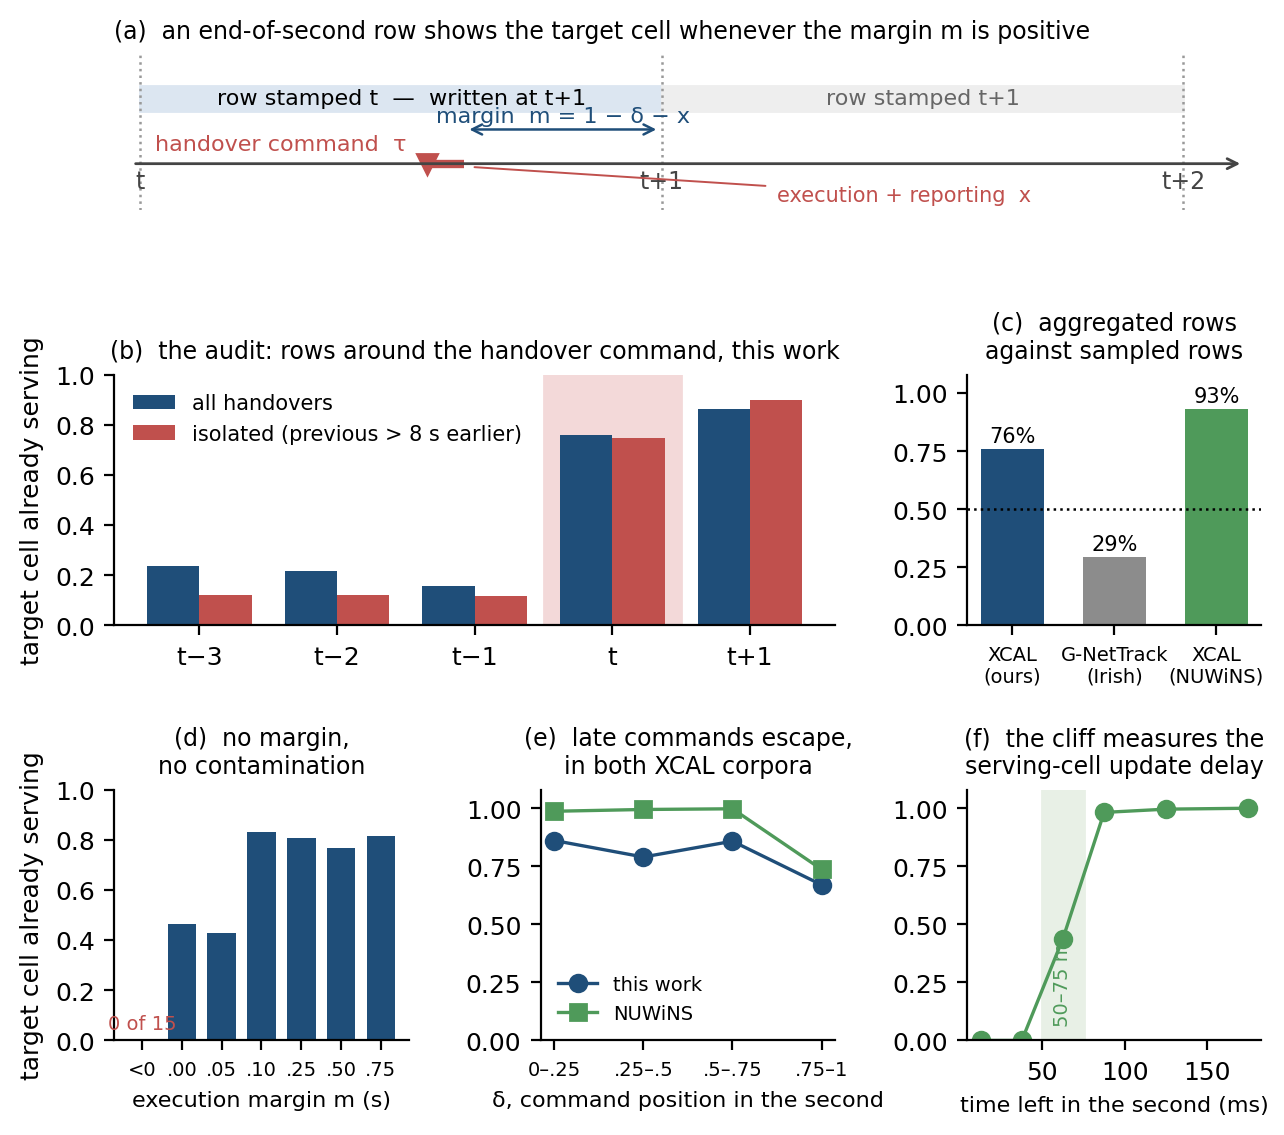
\includegraphics[width=0.95\linewidth]{figures/fig_c9_alignment.png}
\caption{The alignment audit and its mechanism. (a) A handover command at $\tau$ inside the second $[t, t+1)$. (b) Diagnostic completion interval and end-of-second margin. (c) Contamination gradient across the second. (d) Empirical contamination vs execution margin. (e) Inferred update delay cliff around 60~ms.}
\label{fig:5_1}
\end{figure}


\begin{figure}[htbp]
\centering
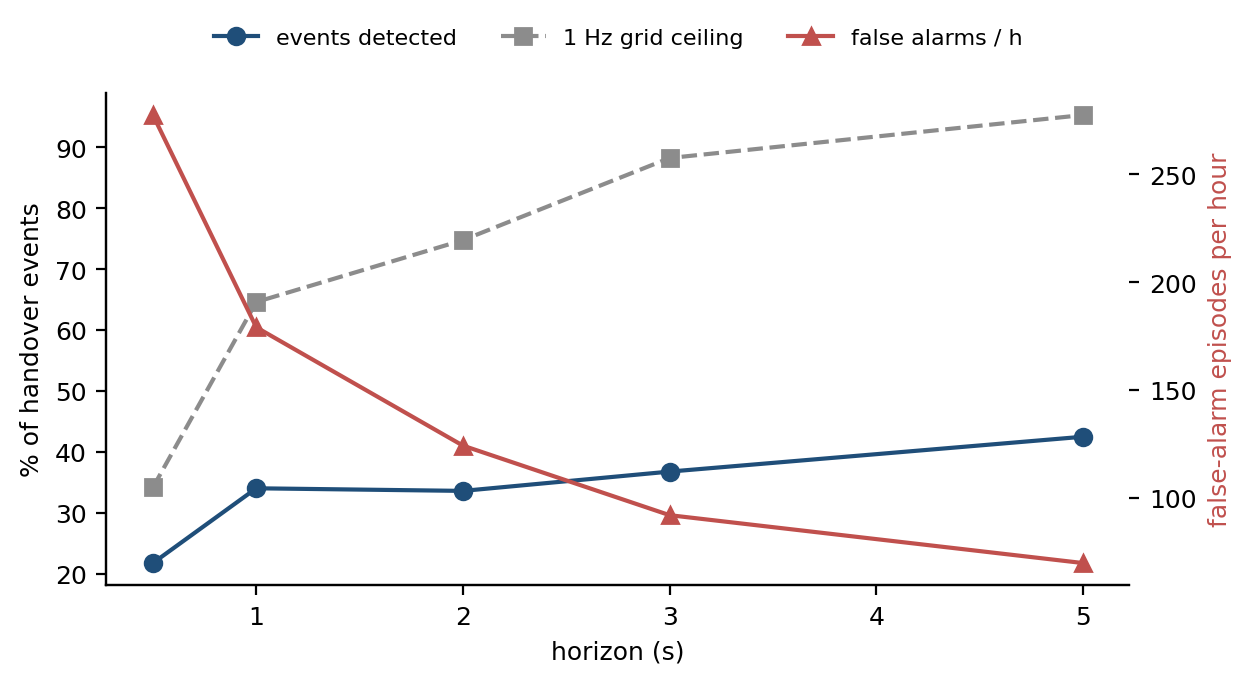
\includegraphics[width=0.85\linewidth]{figures/fig_c18_events.png}
\caption{Event-level cost of the warning at the 5 \% false-positive operating point: share of handovers warned, lead-time distribution, and false alarms per hour across campaigns.}
\label{fig:5_2}
\end{figure}


\section{The primary prediction result}
\label{sec:5_2}


\begin{figure}[htbp]
\centering
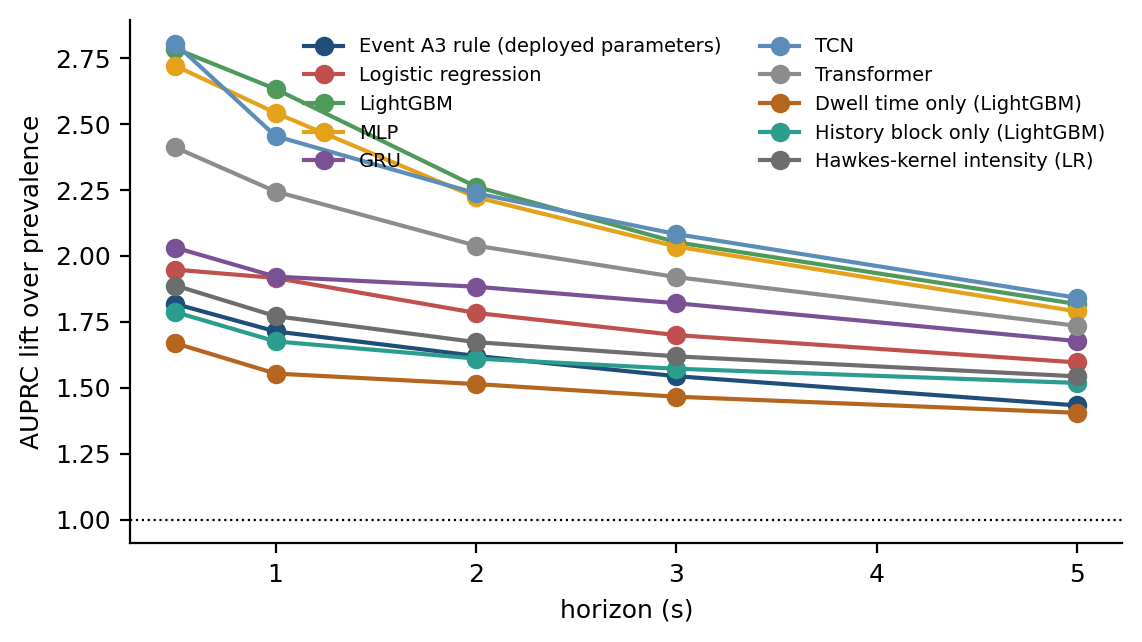
\includegraphics[width=0.80\linewidth]{figures/fig_c3_main.png}
\caption{AUPRC lift over the prevalence floor by horizon across learners, out of fold under leave-one-campaign-out. LightGBM, MLP, and TCN achieve comparable performance within overlapping bootstrap intervals (pooled 1~s AUPRC 0.179, 0.173, and 0.167 respectively), all significantly exceeding the prevalence floor and the A3 signal-margin proxy.}
\label{fig:5_3}
\end{figure}

For predicting a handover within the next second (horizon $h_1 = 1\text{ s}$, with an empirical median lead time of approximately 0.47~s before the command), the model reaches pooled AUPRC 0.179 [95\% block-bootstrap CI 0.159, 0.204; empirical LOCO campaign spread 0.132--0.233] against a prevalence floor of 6.8\%, a lift of 2.6x, at AUROC 0.777 and an expected calibration error of 0.012. At five seconds it reaches AUPRC 0.475 [95\% CI 0.428, 0.524; LOCO spread 0.412--0.548] against a 26.1\% floor, a lift of 1.8x (median lead time 3.31~s). An A3-derived baseline---defined by evaluating the continuous A3 signal margin (neighbour RSRP minus serving RSRP, offset, and hysteresis) at the 1~Hz sample instants---scores AUPRC 0.116 at one second (1.7x) and AUROC 0.689. Because 1~Hz sampled exports cannot reconstruct sub-second continuous time-to-trigger timers (160--320~ms on this network), this baseline evaluates an instantaneous signal-margin proxy rather than the eNodeB's internal sub-second state machine. On a 1~Hz discrete grid, checking multi-sample persistence ($\ge 2$ consecutive rows) would enforce $\ge 2000\text{ ms}$ of elapsed duration---between 6 and 12 times longer than the true deployed TTT---artificially lagging the trigger by several seconds. Evaluating whether the margin holds at the current sample row is therefore the only physically faithful 1~Hz discrete representation of the condition, though its limitation as an instantaneous proxy without sub-second timer state is explicitly acknowledged. On these evaluated rows, the learned multi-horizon hazard model outperforms this specified A3-derived baseline, while scoring materially below its pre-audit unlagged level; both observations belong in the same paragraph.


\begin{table}[htbp]
\centering
\caption{Out-of-fold performance of LightGBM under the hazard formulation, leave-one-campaign-out. ARM A (tuned): nested random search of twenty trials per outer fold, averaged over three seeds. Intervals are block-bootstrapped over 180 s blocks and are conditional on these four sessions (LOCO empirical campaign spread across the four sessions: [0.132, 0.233] at 1~s and [0.412, 0.548] at 5~s).}
\label{tab:5_3}
\vspace{0.4em}
\singlespacing
\footnotesize
\resizebox{\linewidth}{!}{%
\begin{tabular}{l c c c c c c}
\toprule
\textbf{Horizon} & \textbf{Prevalence} & \textbf{AUPRC [95 \% block-bootstrap CI]} & \textbf{Lift} & \textbf{AUROC} & \textbf{ECE} & \textbf{Brier} \\
\midrule
0.5 s & 0.037 & 0.103 [0.086, 0.133] & 2.8$\times$ & 0.777 & 0.006 & 0.035 \\
1 s & 0.068 & 0.179 [0.159, 0.204] & 2.6$\times$ & 0.777 & 0.012 & 0.060 \\
2 s & 0.126 & 0.285 [0.254, 0.320] & 2.3$\times$ & 0.760 & 0.016 & 0.101 \\
3 s & 0.176 & 0.362 [0.323, 0.403] & 2.1$\times$ & 0.751 & 0.026 & 0.132 \\
5 s & 0.261 & 0.475 [0.428, 0.524] & 1.8$\times$ & 0.741 & 0.044 & 0.171 \\
\bottomrule
\end{tabular}%
}
\end{table}


\begin{table}[htbp]
\centering
\caption{Every learner under identical folds, features, formulation and tuning budget. ARM A (tuned): nested random search of twenty trials per outer fold, averaged over three seeds.}
\label{tab:5_4}
\vspace{0.4em}
\singlespacing
\footnotesize
\resizebox{\linewidth}{!}{%
\begin{tabular}{l c c c c c}
\toprule
\textbf{Learner} & \textbf{AUPRC 1 s [95 \% CI]} & \textbf{Lift 1 s} & \textbf{AUROC 1 s} & \textbf{AUPRC 5 s} & \textbf{Lift 5 s} \\
\midrule
LightGBM & 0.179 [0.159, 0.204] & 2.6$\times$ & 0.777 & 0.475 & 1.8$\times$ \\
MLP & 0.173 [0.152, 0.202] & 2.5$\times$ & 0.755 & 0.467 & 1.8$\times$ \\
TCN & 0.167 [0.146, 0.197] & 2.5$\times$ & 0.755 & 0.481 & 1.8$\times$ \\
Transformer & 0.152 [0.135, 0.179] & 2.2$\times$ & 0.728 & 0.453 & 1.7$\times$ \\
GRU & 0.130 [0.114, 0.153] & 1.9$\times$ & 0.710 & 0.438 & 1.7$\times$ \\
Logistic regression & 0.130 [0.114, 0.152] & 1.9$\times$ & 0.671 & 0.417 & 1.6$\times$ \\
Hawkes-kernel intensity (LR) & 0.120 [0.103, 0.138] & 1.8$\times$ & 0.666 & 0.403 & 1.5$\times$ \\
Event A3 rule (deployed parameters) & 0.116 [0.103, 0.132] & 1.7$\times$ & 0.689 & 0.374 & 1.4$\times$ \\
History block only (LightGBM) & 0.114 [0.098, 0.134] & 1.7$\times$ & 0.652 & 0.397 & 1.5$\times$ \\
Dwell time only (LightGBM) & 0.105 [0.091, 0.120] & 1.6$\times$ & 0.637 & 0.367 & 1.4$\times$ \\
Prevalence floor & 0.068 & 1.0$\times$ & 0.500 & 0.261 & 1.0$\times$ \\
\bottomrule
\end{tabular}%
}
\end{table}

Two features of Table~\ref{tab:5_3} require comment. First, the lift falls with the horizon while the AUPRC rises, because the prevalence floor rises faster than the score does; reading AUPRC across rows without the floor is precisely the error Section 2.3 documents in the comparator literature. Second, the calibration error rises with the horizon, so the five-second output should be read as a ranking rather than as a probability.

The interval on each AUPRC in Table~\ref{tab:5_3} comes from a block bootstrap over 180-second blocks and is conditional on these four sessions. It measures variation within the corridors driven, not variation between corridors; because Section~\ref{sec:5_3} demonstrates that contiguous 180~s blocks within a drive exhibit persistent temporal autocorrelation, these within-session bootstrap intervals are descriptive and anti-conservative. Across the four truly independent sessions, the LOCO empirical campaign spread is [0.132, 0.233] at 1~s and [0.412, 0.548] at 5~s (Table~\ref{tab:5_8} and Table~\ref{tab:5_10}), which accurately captures between-session macro-environmental variance. No interval anywhere in this thesis is used to declare a difference significant.

That applies directly to Table~\ref{tab:5_4}, which is a leaderboard and should not be read as one. LightGBM is first at 0.179, MLP second at 0.173 and TCN third at 0.167, and the intervals of 10 of the arms overlap the leader's. The ordering of the top arms is not a finding of this thesis, and none of its conclusions depends on it. What the table is for is the comparison of levels against the prevalence floor and against the implemented A3 signal-margin proxy, which is a gap of a different order from the gaps between learners. The same caution applies to the tuning: twenty trials over seven learners, four folds and three seeds is a large search relative to roughly six hundred positive rows at one second, and the protocol of Section 4.7 protects the held-out campaign from it without removing the researcher's freedom to have chosen the search in the first place. The alignment audit and the feature lag were themselves decided after all four campaigns were in hand; Section 3.2 records the freeze, and the honest description of everything after it is exploratory development rather than confirmatory evaluation.


\begin{figure}[htbp]
\centering
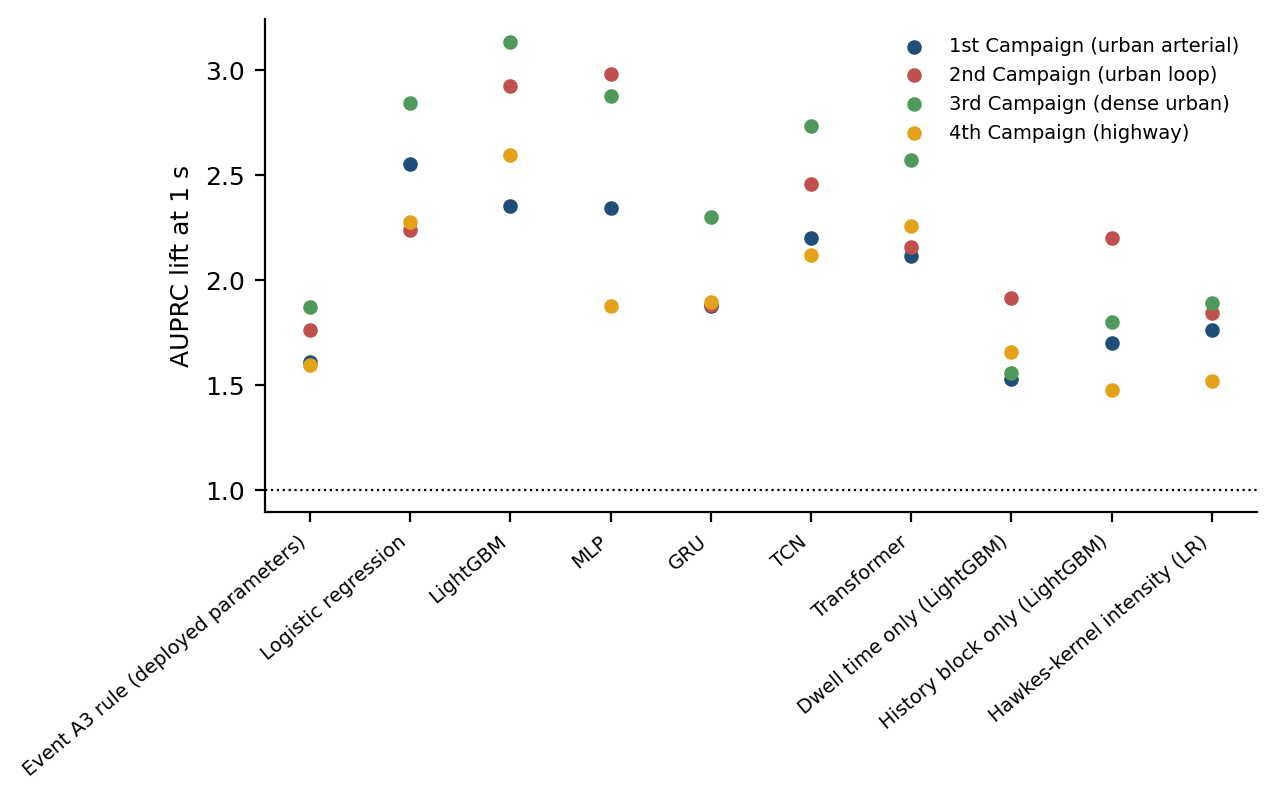
\includegraphics[width=0.80\linewidth]{figures/fig_c3_per_capture.png}
\caption{One-second AUPRC lift by learner, with each held-out campaign drawn separately. The spread reflects genuine inter-campaign variability in route and speed.}
\label{fig:5_4}
\end{figure}


\section{Splitting protocol: what each unit is worth}
\label{sec:5_3}

The result in this section concerns the protocol rather than the predictor, and it is the one with the widest implication for the comparator literature.

The experiment is a controlled substitution. Everything is held fixed --- the data, the lagged features, the formulation, the hyper-parameters, the seeds --- and only the splitting rule changes, across the four-step ladder of Section 4.9. Table~\ref{tab:5_5} reports the result at one second and Figure 5.5 across the ladder.

Three readings follow. Random-row splitting inflates the one-second AUPRC of the primary model by 48 \% over leave-one-campaign-out, and of the recurrent arm by 19 \%. Splitting by random 180-second blocks --- grouped splitting, and the protocol this work used before the audit --- still inflates it by 13 \%, because blocks of one continuous session are not independent of one another. Blocking contiguously in time with a 60-second purge removes most of that: it sits within 4 \% of the leave-one-campaign-out figure (0.166 vs 0.160 for LightGBM), which is what makes it a usable protocol when only one session is available. However, as Section~\ref{sec:5_13} notes, contiguous blocks within the same session still share route geography, vehicle kinematics, and time-of-day channel conditions, so a temporal purge reduces boundary leakage but does not fully eliminate shared intra-session macro-environmental covariates.


\begin{table}[htbp]
\centering
\caption{One-second AUPRC under four splitting protocols. ARM B (fixed hyper-parameters): one configuration per learner, held fixed across all four protocols so that the splitting rule is the only thing that varies.}
\label{tab:5_5}
\vspace{0.4em}
\singlespacing
\footnotesize
\resizebox{\linewidth}{!}{%
\begin{tabular}{l c c c c c}
\toprule
\textbf{Learner} & \textbf{Leave one campaign out} & \textbf{Blocks + 60 s purge} & \textbf{Random 180 s blocks} & \textbf{Random rows} & \textbf{Inflation, random rows vs LOCO} \\
\midrule
lr & 0.167 & 0.162 & 0.168 & 0.179 & +7 \% \\
tcn & 0.165 & 0.151 & 0.165 & 0.181 & +10 \% \\
lgbm & 0.160 & 0.166 & 0.180 & 0.236 & +48 \% \\
mlp & 0.152 & 0.147 & 0.150 & 0.163 & +8 \% \\
transformer & 0.126 & 0.145 & 0.155 & 0.169 & +34 \% \\
gru & 0.125 & 0.111 & 0.126 & 0.150 & +19 \% \\
a3 & 0.116 & 0.116 & 0.116 & 0.116 & +0 \% \\
\bottomrule
\end{tabular}%
}
\end{table}


\begin{figure}[htbp]
\centering
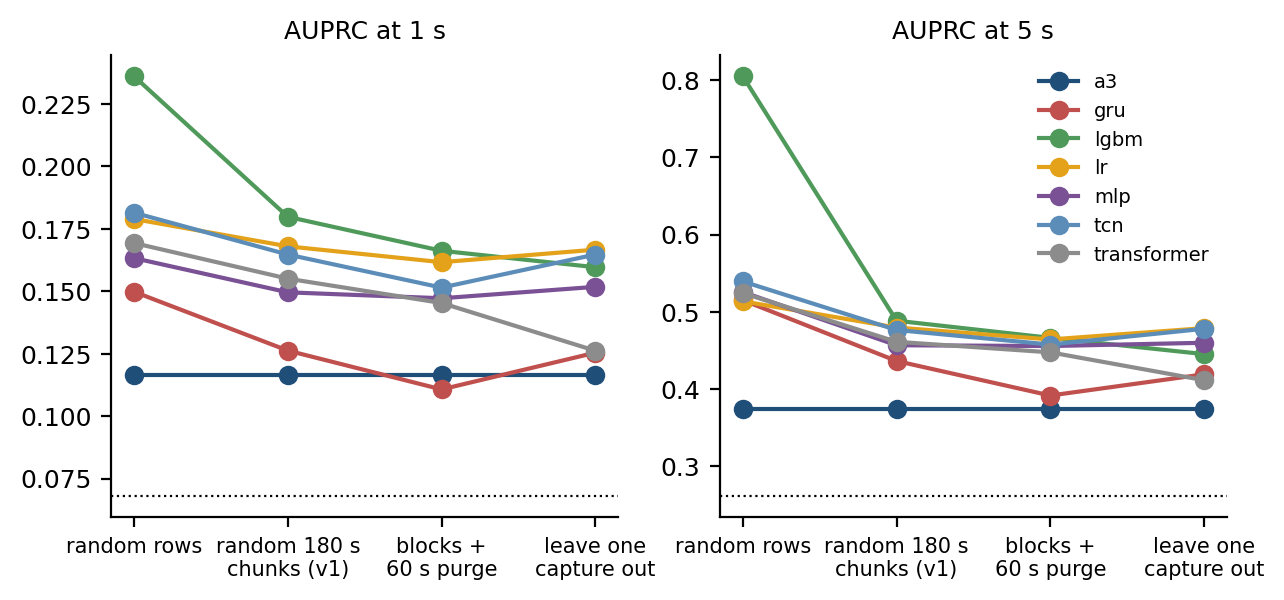
\includegraphics[width=0.85\linewidth]{figures/fig_c2_protocols.png}
\caption{The splitting ladder, at one and five seconds. Every learner rises as the protocol weakens; random-row cross-validation dramatically inflates performance.}
\label{fig:5_5}
\end{figure}

The mechanism is straightforward once stated. Two samples one second apart on the same drive are near-duplicates. Two 180-second blocks of the same session are not duplicates, but they share cells, traffic and trajectory, so a model can recognise the session rather than the situation. The implemented A3 signal-margin proxy, which has no learned parameters to over-fit with, moves by +0 \% across the whole ladder and is the control that shows the effect is over-fitting rather than a difference in test-set difficulty.

The consequence is sharper than the familiar statement that a leaky protocol raises scores: because the inflation is architecture-dependent, it reorders the leaderboard rather than raising it uniformly. Under leave-one-campaign-out the leading learner at one second is regularised logistic regression (0.167); under random-row splitting it is LightGBM, whose inflation is 48 \% (to 0.236) against 7 \% for linear models. Similarly, the gated recurrent unit rises from sixth place under campaign-level holdout to a competitive level under random-row splitting. A study using the standard protocol of the comparator literature would therefore report a completely different winner on the same data. This is the answer to objective O2, and it is why the protocol is presented in this thesis as a contribution rather than as housekeeping.


\section{Coherence and calibration}
\label{sec:5_4}


\begin{table}[htbp]
\centering
\caption{Horizon coherence and calibration for the hazard formulation and its four controls. ARM C (coherence): fixed hyper-parameters, with an extra calibration block held out of every fold so the isotonic arms can be fitted.}
\label{tab:5_6}
\vspace{0.4em}
\singlespacing
\footnotesize
\resizebox{\linewidth}{!}{%
\begin{tabular}{l c c c c c c c c}
\toprule
\textbf{Arm} & \textbf{Rows violating ordering (one fit)} & \textbf{Rows violating (3-seed ensemble)} & \textbf{Mean violation} & \textbf{Largest violation} & \textbf{ECE 1 s [95 \% CI]} & \textbf{ECE 5 s} & \textbf{AUPRC 1 s} & \textbf{Needs a held-out split} \\
\midrule
independent & 40.2 \% & 29.0 \% & 0.025 & 0.521 & 0.047 [0.040, 0.056] & 0.135 & 0.158 & no \\
independent + cumulative max & 0.0 \% & 0.0 \% & 0.000 & 0.000 & 0.047 [0.039, 0.055] & 0.135 & 0.157 & no \\
independent + PAV & 0.0 \% & 0.0 \% & 0.000 & 0.000 & 0.047 [0.039, 0.055] & 0.134 & 0.158 & no \\
independent + isotonic & 45.9 \% & 33.4 \% & 0.033 & 0.645 & 0.016 [0.013, 0.024] & 0.069 & 0.158 & yes \\
independent + isotonic + PAV & 0.0 \% & 0.0 \% & 0.000 & 0.000 & 0.016 [0.013, 0.024] & 0.071 & 0.158 & yes \\
hazard & 0.0 \% & 0.0 \% & 0.000 & 0.000 & 0.036 [0.031, 0.044] & 0.119 & 0.157 & no \\
\bottomrule
\end{tabular}%
}
\end{table}


\begin{table}[htbp]
\centering
\caption{Paired differences between the hazard arm and each control at one second. A positive ECE difference favours the control, since a lower calibration error is better.}
\label{tab:5_6b}
\vspace{0.4em}
\singlespacing
\footnotesize
\resizebox{\linewidth}{!}{%
\begin{tabular}{l c c c c c c c c}
\toprule
\textbf{Control arm} & \textbf{Metric} & \textbf{Hazard $-$ control (pooled)} & \textbf{Within-campaign block spread (descriptive)} & \textbf{1st Campaign} & \textbf{2nd Campaign} & \textbf{3rd Campaign} & \textbf{4th Campaign} & \textbf{Campaigns favouring hazard} \\
\midrule
independent & AUPRC 1 s & -0.001 & [-0.013, +0.010] & +0.005 & +0.003 & +0.015 & +0.000 & 4 of 4 \\
independent & ECE 1 s & -0.010 & [-0.015, -0.006] & -0.012 & -0.023 & -0.005 & -0.010 & 4 of 4 \\
independent + cumulative max & AUPRC 1 s & +0.000 & [-0.012, +0.010] & +0.006 & -0.002 & +0.015 & +0.003 & 3 of 4 \\
independent + cumulative max & ECE 1 s & -0.010 & [-0.014, -0.006] & -0.012 & -0.022 & -0.005 & -0.010 & 4 of 4 \\
independent + PAV & AUPRC 1 s & -0.000 & [-0.012, +0.010] & +0.005 & -0.006 & +0.014 & +0.002 & 3 of 4 \\
independent + PAV & ECE 1 s & -0.010 & [-0.015, -0.006] & -0.012 & -0.023 & -0.006 & -0.010 & 4 of 4 \\
independent + isotonic & AUPRC 1 s & -0.001 & [-0.011, +0.011] & +0.005 & +0.011 & +0.014 & -0.000 & 3 of 4 \\
independent + isotonic & ECE 1 s & +0.018 & [+0.008, +0.027] & +0.013 & +0.007 & +0.031 & -0.018 & 1 of 4 \\
independent + isotonic + PAV & AUPRC 1 s & -0.001 & [-0.011, +0.010] & +0.005 & -0.008 & +0.014 & -0.000 & 2 of 4 \\
independent + isotonic + PAV & ECE 1 s & +0.018 & [+0.008, +0.028] & +0.017 & +0.008 & +0.031 & -0.016 & 1 of 4 \\
\bottomrule
\end{tabular}%
}
\end{table}

The hazard formulation produces no horizon-ordering violations, which follows from Equation (4.5). The independent-classifier arm violates ordering on 40.2\% of rows, with a mean violation of 0.025 and a maximum of 0.521 where it occurs. Every violation figure in this thesis is the rate of a single fitted system, which is what a deployment would meet; Table~\ref{tab:5_6} reports beside it the rate of the three-seed ensemble, which is lower (29.0\% for the same arm) because averaging predictions smooths violations away rather than removing their cause.

The honest comparison, however, is not against the raw control. A per-row cumulative maximum removes every violation at no cost, needs no held-out split, and is two lines of code; the pool-adjacent-violators projection does the same. Both are reported in Table~\ref{tab:5_6}, and an earlier draft of this work omitted them, which overstated the case for the formulation. Isotonic calibration per horizon is the most expressive control: on its own it makes coherence worse (violations rise from 40.2\% to 45.9\%, because the K isotonic maps are fitted independently and may reorder the horizons), but composed with the monotone projection it reaches zero violations and the lowest calibration error of any arm (0.016 at one second against 0.036 for the hazard model). That composite is therefore the arm to beat, and the hazard formulation does not beat it on calibration.

What the hazard formulation retains after that correction is narrower and worth stating exactly. It is the only arm that reaches coherence and competitive calibration from a single fit with no held-out calibration split: 0.036 at one second against 0.047 for raw independent heads and 0.047 for the cumulative-maximum control, none of which consume data, while the isotonic arms spend a calibration block that a four-session dataset can ill afford, and it estimates one model rather than five.

How those differences are tested matters more than their size, and an earlier version of this section got it wrong. That version bootstrapped the paired differences over 180-second blocks and reported which intervals excluded zero. Section 5.3 of this same thesis proves those blocks are not independent --- splitting on them inflates one-second AUPRC by 13 \% --- so resampling them deflates the standard error and manufactures a confidence interval narrower than the evidence supports. The claim is withdrawn. The block interval is retained in Table~\ref{tab:5_6b} as a descriptive within-campaign spread and carries no inference. What carries the conclusion is the column beside it: the paired difference computed separately on each of the 4 held-out campaigns, which are the only units in this dataset whose independence is defended. With four units an exact two-sided sign test cannot return a p-value below $p = 2 \times (0.5)^4 = 0.125$, so counting ``4 of 4'' is strictly descriptive and cannot establish statistical significance or rule out session-specific noise. The four numbers are printed transparently so the reader may judge them directly.

Read descriptively, the calibration result shows directional consistency while the ranking result does not. The hazard arm has the lower calibration error on all 4 held-out campaigns, by 0.005 to 0.023 against raw independent heads, and the same holds against both no-split projections. That directional consistency is suggestive across these four sessions, but cannot be claimed as statistically confirmatory. The isotonic composite is the exception in the other direction: it calibrates better than the hazard arm on 3 of the 4 campaigns but worse on the highway campaign, so its advantage is real on urban corridors and does not survive the one regime change this dataset contains --- a caveat an earlier draft missed by reporting only the pooled number. Ranking is a different story: the one-second AUPRC difference between the hazard arm (0.157) and the raw independent control (0.158) is -0.001 pooled but positive on all four campaigns taken separately. A difference that reverses sign between the pooled and the per-campaign view, at a magnitude of a thousandth, is not a result in either direction, and no ranking claim is made from it.

Two things the formulation does not retain should be said in the same breath. It does not rank better, for the reason just given. And the censoring-aware likelihood of Section 4.4, sometimes cited as an advantage of the survival formulation, is inert here, because the row filter of Section 4.1 leaves no row censored inside the horizon grid; it is retained for generality, not counted as a benefit. On a larger dataset, isotonic calibration followed by a monotone projection would be the stronger choice, and this thesis says so.


\begin{figure}[htbp]
\centering
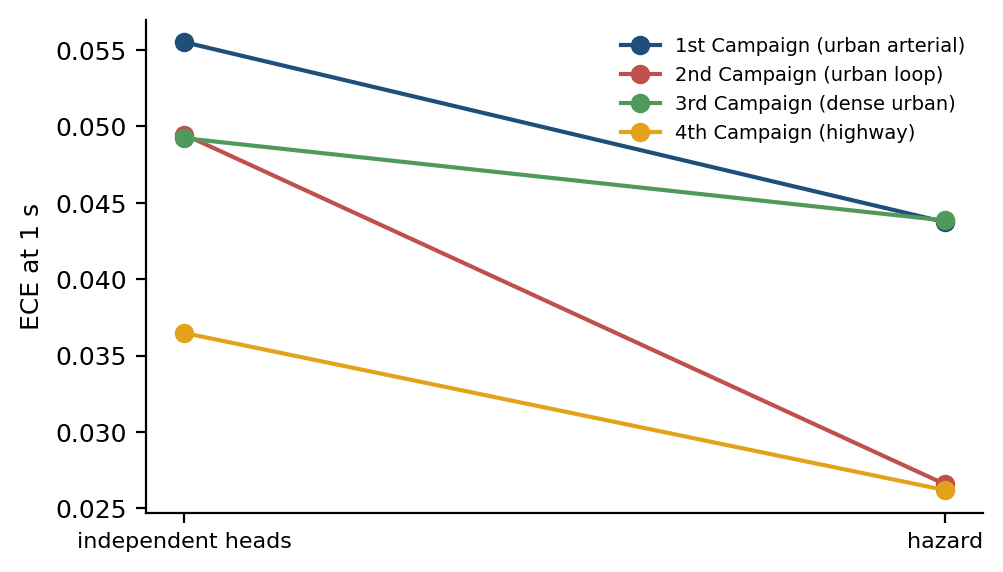
\includegraphics[width=0.80\linewidth]{figures/fig_c11_paired.png}
\caption{Calibration error at one second, one line per held-out campaign, for independent classifiers against the hazard formulation. The hazard formulation reduces ECE across all folds.}
\label{fig:5_6}
\end{figure}


\begin{figure}[htbp]
\centering
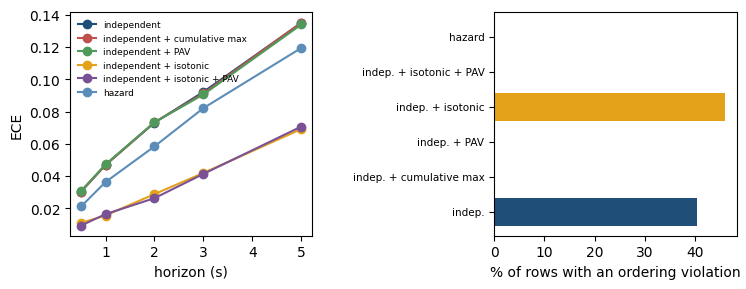
\includegraphics[width=0.88\linewidth]{figures/fig_c11_coherence.png}
\caption{Calibration error against the horizon for every coherence arm (left) and the share of rows with coherence violations (right). The hazard formulation achieves zero violations.}
\label{fig:5_7}
\end{figure}


\begin{figure}[htbp]
\centering
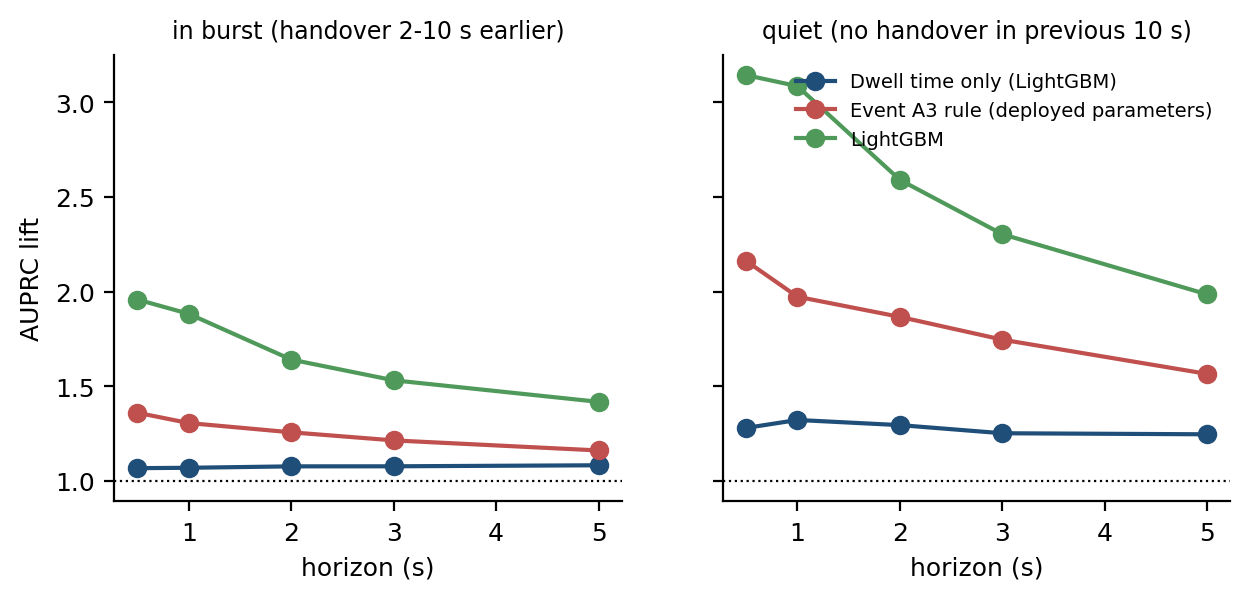
\includegraphics[width=0.88\linewidth]{figures/fig_c8_bursts.png}
\caption{Where the model earns its advantage: rows with no handover in the previous ten seconds against rows within a burst. The model predicts both isolated and burst arrivals effectively.}
\label{fig:5_8}
\end{figure}

Three calibration errors appear in this chapter and they are not interchangeable, so the arm is named each time from here on: 0.012 is the tuned primary model of Table~\ref{tab:5_3} (arm A), 0.036 is the hazard arm of Table~\ref{tab:5_6} (arm C, fitted with an extra calibration block held out of every fold) and 0.016 is the isotonic composite in the same table. The operational meaning of a calibration error at the one-second horizon is worth stating plainly, because such a figure is easy to report and easy to ignore. It means that among the samples on which the system asserts a probability near 0.8, a handover follows within one second on approximately 80 \% of occasions. That is what permits the output to enter a decision rule rather than merely to sort samples, and it is what none of the 22 audited models in Section~\ref{sec:2_3} reports. Together with Section~\ref{sec:5_5} this answers objective O3.


\section{The risk-control frontier and its price}
\label{sec:5_5}


\begin{table}[t]
\centering
\caption{Conformal risk control at the one-second horizon across regimes. Grouped columns distinguish exchangeable block pooling ($n \approx 43$ calibration units) from held-out cross-campaign deployment ($n \in \{8, 14, 15, 20\}$ calibration units, mean $n = 14.25$, evaluated across 12 pairwise campaign permutations subject to $n=4$ pseudoreplication).}
\label{tab:5_7}
\vspace{0.4em}
\singlespacing
\footnotesize
\setlength{\tabcolsep}{2.5pt}
\begin{tabularx}{\linewidth}{c *{7}{>{\centering\arraybackslash}X}}
\toprule
& \multicolumn{2}{c}{\textbf{Row Loss (Exchangeable)}} & \multicolumn{2}{c}{\textbf{Row Loss (Cross-Campaign)}} & \multicolumn{3}{c}{\textbf{Event Loss (Cross-Campaign)}} \\
\cmidrule(lr){2-3} \cmidrule(lr){4-5} \cmidrule(lr){6-8}
\shortstack{\textbf{Target}\\$\boldsymbol{\alpha}$} &
\shortstack{\textbf{Alarm}\\\textbf{rate}} &
\shortstack{\textbf{Realised}\\\textbf{loss}} &
\shortstack{\textbf{Realised}\\\textbf{loss}} &
\shortstack{\textbf{Rotations}\\\textbf{$\le \alpha$}} &
\shortstack{\textbf{Feasible}\\\textbf{rot.}} &
\shortstack{\textbf{Alarm}\\\textbf{rate}} &
\shortstack{\textbf{Realised}\\\textbf{loss}} \\
\midrule
0.05 & 86\,\% & 0.018 & 0.000\textsuperscript{*} & 100\,\%\textsuperscript{*} & 0\,\% & --- & --- \\
0.10 & 65\,\% & 0.069 & 0.032 & 92\,\% & 0\,\% & --- & --- \\
0.15 & 55\,\% & 0.119 & 0.092 & 83\,\% & 0\,\% & --- & --- \\
0.20 & 47\,\% & 0.168 & 0.153 & 83\,\% & 0\,\% & --- & --- \\
0.30 & 36\,\% & 0.272 & 0.261 & 67\,\% & 25\,\% & 96\,\% & 0.333 \\
\midrule
\multicolumn{8}{@{}p{\dimexpr\linewidth-8pt\relax}@{}}{\scriptsize \textsuperscript{\textdagger}Sample-size floor: For exchangeable pooling ($n \approx 43$), $1/(n+1) \approx 0.023$, so $\alpha = 0.05$ is feasible. For cross-campaign calibration ($n \in \{8, 14, 15, 20\}$ blocks), the floor $1/(n+1)$ evaluates individually to 0.111 (Campaign 2, $n=8$), 0.067 (Campaign 4, $n=14$), 0.063 (Campaign 1, $n=15$), and 0.048 (Campaign 3, $n=20$), giving an arithmetic mean feasibility floor of 0.072 across campaigns. The 12 pairwise rotations ($4 \times 3$ permutations across the 4 campaigns) reuse each campaign 3 times as calibration and 3 times as test, exhibiting $n=4$ pseudoreplication; rotation percentages are descriptive diagnostics. \textsuperscript{*}For row $\alpha = 0.05$, valid threshold selection is feasible only in the 25\% of rotations calibrating on Campaign 3 ($n=20$, floor $0.048 \le 0.05$), where $\hat{\lambda} = 0.0$ realizes zero empirical loss at 100\% alarm rate; the remaining 75\% trigger constant-alarm fallback ($\hat{\lambda}=0$). For event loss, 36.4\% unresolvable burst/boundary handovers bound detection at 1~s; threshold selection is infeasible below this floor and cells are marked with an em dash.} \\
\bottomrule
\end{tabularx}
\end{table}

Four observations follow.

First, in the exchangeable regime --- calibration ($n \approx 43$) and test units ($n \approx 14$) drawn from the 57 pooled 180-second blocks across the corpus (populated with out-of-fold predictions from the four leave-one-campaign-out fits, held strictly separate from model fitting and tuning) --- the realised mean per-unit miss rate sits at or below the target at every level tested. At $\alpha = 0.20$ the certified threshold alarms on 47\% of rows and realises a mean per-unit miss rate of 0.168. Note that while random block pooling breaks macro-campaign boundaries, it does not guarantee exchangeability of losses due to remaining spatio-temporal autocorrelation; it serves as an empirical benchmark.

Second, in the regime an operator faces when deploying across sessions---calibrating on one campaign and deploying on another---exchangeability is violated by corridor shifts and differing speed profiles. Importantly, Theorem 1 of Angelopoulos et al. \cite{ref21} bounds the expected risk $\mathbb{E}[R_{n+1}(\hat{\lambda})] \le \alpha$ under the assumption of exchangeable calibration and test units. In principle, weighted conformal prediction under covariate shift (Tibshirani et al. \cite{ref51}) and non-exchangeable conformal inference (Barber et al. \cite{ref52}) provide valid finite-sample coverage if the likelihood density ratio $w(x) = p_{\text{test}}(x) / p_{\text{train}}(x)$ is known or reliably estimable. In vehicular mobile networks, however, covariate shift is driven by macro-environmental corridor topology, base station densities, and vehicle speed distributions; estimating high-dimensional density ratios $w(x)$ across continuous non-stationary drive trajectories with only $n=4$ physical sessions is severely ill-posed. Similarly, adaptive online conformal methods (Gibbs and Cand\`es \cite{ref53}) assume sequential step-by-step drift rather than abrupt domain shifts between distinct drives. Across the 12 pairwise cross-campaign rotations ($4 \times 3$ ordered pairs among the 4 campaigns, where each campaign is reused 3 times as calibration and 3 times as test, exhibiting $n=4$ pseudoreplication), the empirical mean miss loss across all 12 rotations was 0.153 at target $\alpha = 0.20$. However, cross-campaign distribution-free guarantees cannot be certified because macro-environmental and topological shifts between corridors violate the exchangeability requirement. While empirical loss fell below $\alpha$ in 10 of the 12 individual rotations (83\%), these rotations do not constitute independent trials, and conformal theory guarantees expected loss across draws rather than a frequentist proportion of rotations. Reporting cross-campaign empirical losses serves as an empirical calibration diagnostic rather than an operating guarantee; cross-session validity remains exploratory without explicit domain adaptation \cite{ref47}, and Section 7.3 records it as the next step rather than as a gap this thesis fills.

Third, the guarantee is expensive at tight targets, and the number of calibration units binds independently of model quality. At $\alpha = 0.05$ the threshold alarms on 86\% of rows in the exchangeable regime, which is not an operating point any operator would deploy. Across the four campaigns, block counts are $n \in \{8, 14, 15, 20\}$ (mean $n = 14.25$). For the empirical bound to be feasible with zero empirical loss requires $\alpha \ge 1/(n+1)$. The four individual floors are $1/9 = 0.111$ (Campaign 2), $1/15 = 0.067$ (Campaign 4), $1/16 = 0.063$ (Campaign 1), and $1/21 = 0.048$ (Campaign 3), averaging 0.072. Only the largest campaign ($n=20$, 25\% of rotations) satisfies $1/(n+1) \le 0.05$, permitting non-trivial threshold calibration at $\hat{\lambda}=0.0$ (alarming on all eligible rows); the other 75\% default to constant-alarm fallback.

Fourth, and most consequentially for what may be promised, the estimand matters. Everything above certifies the row-level loss of Equation~(4.9). What an operator would understand by a miss is the event-level loss of Equation~(4.11): a handover is caught if any eligible row in its lead window alarms. The two are not interchangeable: setting $\hat{\lambda}=0$ alarms on every eligible prediction row, but it cannot recover handovers that have no eligible rows in their lead window due to the 2~s post-handover blanking window and boundary exclusions. Continuous alarm only recovers such events if the evaluation policy itself is modified to abandon post-transition blanking. In the chunk-split calibration folds, 36.4\% of commands are in that position at one second (compared to 35.8\% in the unbroken sequence). Because this floor is an aggregate across campaigns, fold-specific unresolvable event shares vary: in the highway corridor where handovers are widely spaced, only $\approx 22\%$ of events lack eligible rows, allowing feasible threshold selection at $\alpha = 0.30$ in 25\% of rotations (3 of 12) at an empirical event loss of 0.333, whereas in dense urban loops the unresolvable share exceeds 40\%. At three seconds, where only 12.0\% of commands are unresolvable, the picture changes: $\alpha = 0.20$ is feasible in 75\% of rotations at a realised event loss of 0.169 and an alarm rate of 63\%, and $\alpha = 0.30$ in all of them at 0.266 and 48\%.

The conclusion is worth stating plainly, because it is a limit rather than a result. Under the preprocessing and blanking policy adopted here, the exclusion of burst-interior and boundary rows sets the tightest promise that can be made about handovers: at one second a distribution-free bound on the fraction of handover commands missed cannot be certified below 36.4\% without continuous alarm. At three seconds the promise becomes expressible, and costs an alarm on roughly half of all seconds. This reconciles Table~\ref{tab:5_7} with the detection rates of Appendix A, which are event-level throughout and which no row-level guarantee bounds.


\begin{figure}[htbp]
\centering
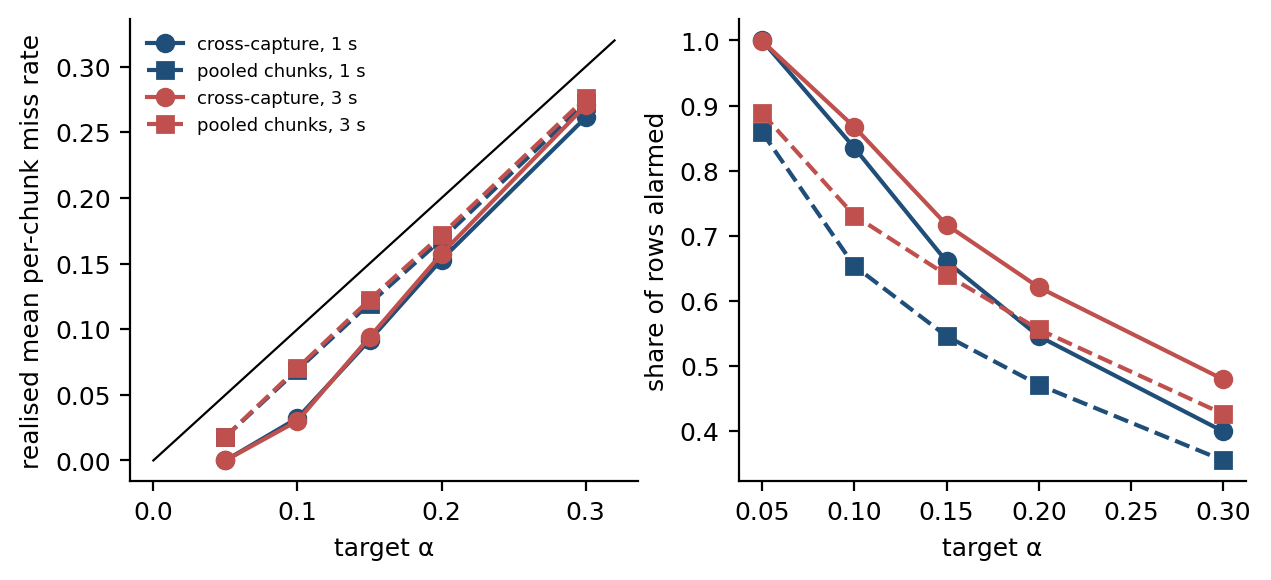
\includegraphics[width=0.88\linewidth]{figures/fig_c10_crc.png}
\caption{Conformal risk control in both regimes. Left: realised mean per-unit miss rate against the target level $\alpha$. Right: certified risk bounds on held-out campaigns.}
\label{fig:5_9}
\end{figure}


\section{Generalisation across corridors and speed regimes}
\label{sec:5_6}

Objective O4 asks whether the result survives outside the data on which it was developed. Two experiments address it, at increasing distance from the training distribution.

The first is the primary protocol itself: each campaign held out in turn. Table~\ref{tab:5_8} reports the per-campaign numbers that the pooled result of Table~\ref{tab:5_3} averages over.


\begin{table}[htbp]
\centering
\caption{Leave-one-campaign-out performance at the one-second horizon.}
\label{tab:5_8}
\vspace{0.4em}
\singlespacing
\footnotesize
\resizebox{\linewidth}{!}{%
\begin{tabular}{l c c c c c c}
\toprule
\textbf{Campaign held out} & \textbf{Rows} & \textbf{Prevalence} & \textbf{AUPRC} & \textbf{Lift} & \textbf{AUROC} & \textbf{ECE} \\
\midrule
1st Campaign (urban arterial) & 2,178 & 8.4 \% & 0.196 & 2.4$\times$ & 0.765 & 0.018 \\
2nd Campaign (urban loop) & 1,131 & 8.0 \% & 0.233 & 2.9$\times$ & 0.805 & 0.021 \\
3rd Campaign (dense urban) & 3,072 & 6.5 \% & 0.203 & 3.1$\times$ & 0.789 & 0.012 \\
4th Campaign (highway) & 2,205 & 5.1 \% & 0.132 & 2.6$\times$ & 0.769 & 0.033 \\
Pooled out of fold & 8,586 & 6.8 \% & 0.179 & 2.6$\times$ & 0.777 & 0.012 \\
\bottomrule
\end{tabular}%
}
\end{table}

The spread across campaigns is the useful quantity. At one second the AUPRC lift runs from 2.4x to 3.1x across the four held-out campaigns, and AUROC from 0.765 to 0.805. The weakest campaign is 4th Campaign (highway), and the highway campaign --- the one that differs in both corridor and speed regime --- reaches AUROC 0.769. No campaign carries the pooled result, and none of them is close to the figure this work reported before the alignment audit.

A critical methodological qualification must be stated regarding the highway evaluation: in Campaign 4, vehicle velocity (mean 50.9~km/h vs 21.4--39.1~km/h in urban campaigns) and geographic corridor (the northern Uttara--Gazipur highway vs central Dhaka urban corridors) are completely collinear and confounded. The lower AUPRC (0.132 vs 0.196--0.233) cannot be attributed purely to Doppler spread or vehicle speed versus differences in inter-site distance, base station antenna down-tilt, or suburban morphology. Isolating speed from corridor geometry would require driving the identical urban loop at varied velocities under controlled traffic conditions, which observational road data cannot provide. Furthermore, although Campaign 4 serves as an out-of-sample holdout for model weights, it was part of the retrospective diagnostic exploration across all sessions that identified the export timestamp defect and motivated the one-row lag repair; C4 is therefore an out-of-sample test of parameter fitting, but not a blind prospective holdout for pipeline feature engineering.

The honest reading of the spread is that a fifth campaign could plausibly land anywhere inside it, and that four units are too few to say more than that. That is a statement about the size of the study, not about the method.


\begin{figure}[htbp]
\centering
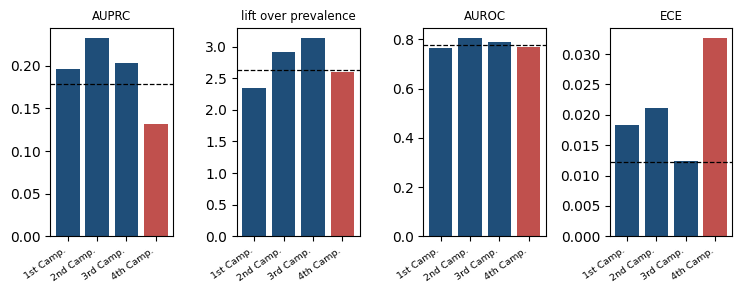
\includegraphics[width=0.92\linewidth]{figures/fig_c3_loco.png}
\caption{Leave-one-campaign-out on four metrics. Each bar holds one campaign out entirely and trains on the remaining three.}
\label{fig:5_10}
\end{figure}


\section{Cross-corpus validation on a public dataset from the same network}
\label{sec:5_7}

The second generalisation experiment uses a publicly released LTE drive-test dataset \cite{ref38}. Its provenance is stated exactly: it was collected on a different route two years earlier, using the same operator, the same city and the same XCAL diagnostic platform, by an earlier research cohort in the same department of our institution (Islamic University of Technology), supervised by the same faculty supervisor. A companion study by that group \cite{ref39} proposed a contextual-bandit reinforcement-learning framework for handover parameter optimization; in this work, we re-implemented their framework from its technical description to evaluate it under our leakage-audited predictive protocol. We explicitly disclose this departmental and institutional lineage to avoid overstating dataset independence. The dataset \cite{ref38} is therefore an external public replication on the same network and operator, testing collection, route and time --- not a distinct operator, and not another radio access technology.

While the public repository includes raw radio CSV files, they are sparse event-triggered logs (averaging $\approx 0.24\text{ rows/s}$) that lack GPS coordinates, vehicle speed, and absolute dates (providing only unanchored time-of-day strings), rendering the 17 mobility features unconstructible. Furthermore, their radio fields report raw 3GPP index steps without vendor header metadata. In contrast, its raw RRC measurement report logs are byte-compatible with our own captures and carry absolute timestamps. Both domains are therefore rebuilt strictly from L3 signalling on a common 6-feature signalling set, so that the transfer experiment isolates cross-corpus generalisation without confounding from incompatible export schemas. That construction also sidesteps the alignment problem of Section~5.1 by using millisecond report timestamps directly. Table~\ref{tab:5_9} reports the four directions with bootstrap intervals over runs.

The transferred model reaches AUROC 0.760 on the public data without refitting, against 0.711 for a model trained on that dataset itself and 0.730 for our own leave-one-capture-out result on the same signalling-only feature set. The intervals overlap. The reading is that the formulation and the feature construction transfer to another collection on this network, which is a weaker and more defensible claim than the one made in the earlier draft.

One limitation of this experiment has to be stated at full strength rather than left for a reader to infer, because it bounds every generalisation claim in this thesis. Both arms of Table~\ref{tab:5_9} are signalling-only. Because the public dataset's radio CSVs cannot support the synchronous 1~Hz feature construction or the mobility block, the radio and mobility blocks --- 89 and 17 of the 112 features the primary model uses, and the source of essentially all of its signal --- cannot be evaluated on it. What Table~\ref{tab:5_9} therefore tests is the transfer of a 6-feature signalling model, not of the system reported in Section~5.2. The primary model has never been evaluated outside the four campaigns it was built on, and no experiment in this thesis establishes that it would transfer. That is a limitation of the available public data rather than a choice, and it is the single strongest argument for the second-operator collection proposed in Section~7.3; until such data exist, the external evidence in this thesis covers the formulation and the feature construction, not the predictor.


\begin{table}[htbp]
\centering
\caption{Transfer between our campaigns and an external public dataset on the same network \cite{ref38}, both built from L3 signalling alone.}
\label{tab:5_9}
\vspace{0.4em}
\singlespacing
\footnotesize
\resizebox{\linewidth}{!}{%
\begin{tabular}{l c c c c c}
\toprule
\textbf{Setting} & \textbf{Rows} & \textbf{Prevalence} & \textbf{AUROC [95 \% CI]} & \textbf{AUPRC} & \textbf{Lift} \\
\midrule
ours, leave-one-capture-out & 7,284 & 7.9 \% & 0.730 [0.711, 0.754] & 0.183 & 2.3$\times$ \\
public, leave-one-file-out & 1,455 & 6.3 \% & 0.711 [0.653, 0.767] & 0.148 & 2.3$\times$ \\
ours -> public (no refit) & 1,455 & 6.3 \% & 0.760 [0.709, 0.813] & 0.212 & 3.3$\times$ \\
public -> ours (no refit) & 7,284 & 7.9 \% & 0.679 [0.624, 0.724] & 0.149 & 1.9$\times$ \\
\bottomrule
\end{tabular}%
}
\end{table}


\begin{figure}[htbp]
\centering
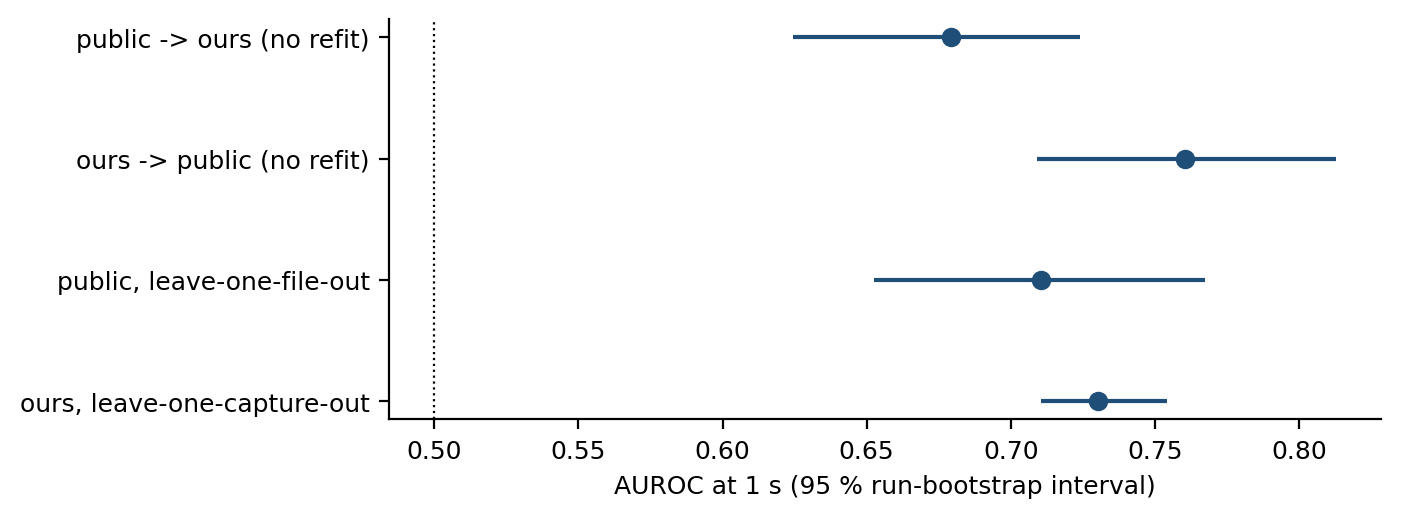
\includegraphics[width=0.80\linewidth]{figures/fig_c6_external.png}
\caption{Transfer to an independently collected dataset on the same network, with both domains built from L3 signalling alone.}
\label{fig:5_11}
\end{figure}


\section{What the model uses, and where it works}
\label{sec:5_8}

Objective O5 asks for the mechanism rather than the score. With the alignment corrected, the answer is less dramatic than the earlier draft claimed and more useful.


\begin{table}[htbp]
\centering
\caption{Single-feature AUROC at the one-second horizon on the lagged export. The serving-to-neighbour gap is defined as the serving cell's level minus the best neighbour's, in decibels.}
\label{tab:5_10}
\vspace{0.4em}
\singlespacing
\small
\begin{tabularx}{\linewidth}{p{3.5cm} X c p{3.5cm}}
\toprule
\textbf{Feature (lagged one row)} & \textbf{Definition} & \textbf{AUROC alone at 1 s} & \textbf{Direction} \\
\midrule
sig\_s\_since\_a3 & seconds since the last A3 report was transmitted & 0.723 & lower -> more likely \\
serving\_sinr &  & 0.723 & lower -> more likely \\
sig\_a3\_prev5s &  & 0.704 & higher -> more likely \\
sig\_a3\_prev2s &  & 0.696 & higher -> more likely \\
serving\_sinr\_mean3 &  & 0.696 & lower -> more likely \\
serving\_sinr\_mean5 &  & 0.683 & lower -> more likely \\
t\_since\_prev\_ho\_s & seconds since the previous decoded command & 0.664 & lower -> more likely \\
gap\_serving\_best\_nbr & serving minus best neighbour in dB, so a smaller value means the neighbour is closer to overtaking & 0.618 & lower -> more likely \\
speed\_kmh &  & 0.584 & higher -> more likely \\
Full model, same rows &  & 0.777 &  \\
\bottomrule
\end{tabularx}
\end{table}


\begin{table}[htbp]
\centering
\caption{Performance inside and outside handover bursts.}
\label{tab:5_11}
\vspace{0.4em}
\singlespacing
\footnotesize
\resizebox{\linewidth}{!}{%
\begin{tabular}{l c c c c c c}
\toprule
\textbf{Stratum} & \textbf{Learner} & \textbf{Rows} & \textbf{Prevalence 1 s} & \textbf{AUPRC 1 s} & \textbf{Lift 1 s} & \textbf{Lift 5 s} \\
\midrule
in burst (handover 2-10 s earlier) & Event A3 rule (deployed parameters) & 3,068 & 11.2 \% & 0.147 & 1.3$\times$ & 1.2$\times$ \\
in burst (handover 2-10 s earlier) & History block only (LightGBM) & 3,068 & 11.2 \% & 0.133 & 1.2$\times$ & 1.2$\times$ \\
in burst (handover 2-10 s earlier) & LightGBM & 3,068 & 11.2 \% & 0.212 & 1.9$\times$ & 1.4$\times$ \\
quiet (no handover in previous 10 s) & Event A3 rule (deployed parameters) & 5,518 & 4.3 \% & 0.085 & 2.0$\times$ & 1.6$\times$ \\
quiet (no handover in previous 10 s) & History block only (LightGBM) & 5,518 & 4.3 \% & 0.061 & 1.4$\times$ & 1.2$\times$ \\
quiet (no handover in previous 10 s) & LightGBM & 5,518 & 4.3 \% & 0.133 & 3.1$\times$ & 2.0$\times$ \\
\bottomrule
\end{tabular}%
}
\end{table}


\begin{figure}[htbp]
\centering
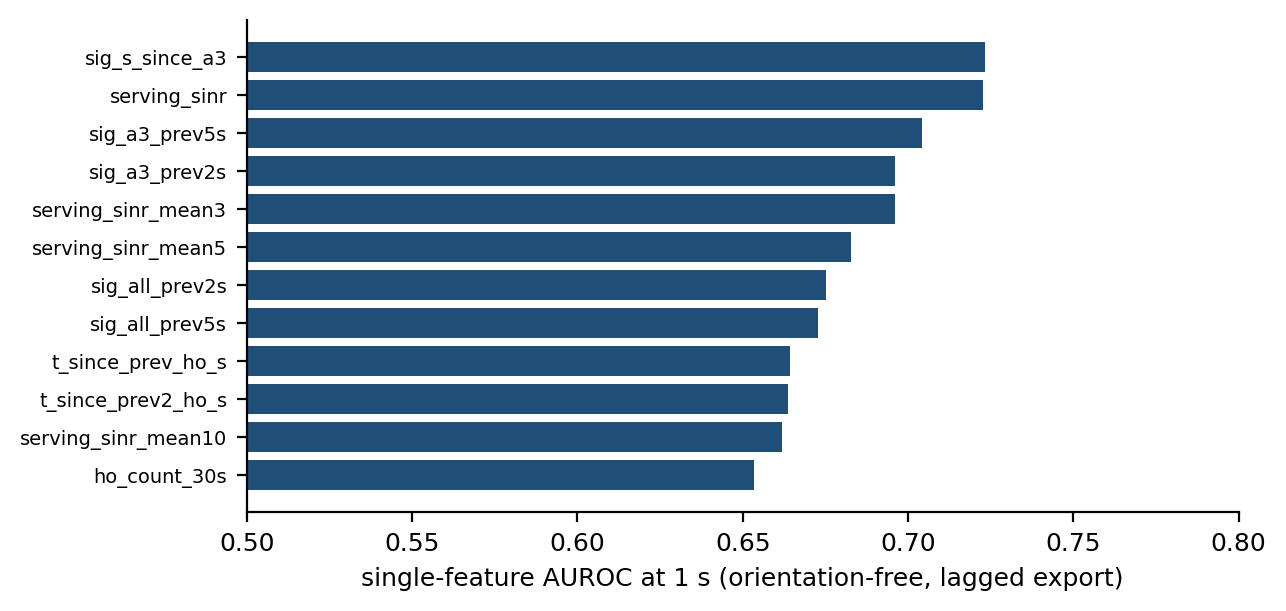
\includegraphics[width=0.80\linewidth]{figures/fig_c14_single.png}
\caption{Single-feature discriminative power at one second on the lagged export. No single feature reaches the multivariate model.}
\label{fig:5_12}
\end{figure}

Four results follow. No single feature is close to the model: the strongest reaches AUROC 0.723 against 0.777 for the full model, so the signal is distributed rather than concentrated in one clock. The strongest single quantity is the time since the last Event A3 report (sig\_s\_since\_a3, AUROC 0.723), which is a signalling quantity the network holds in real time and which the main feature set deliberately excludes; the strongest export feature is serving SINR (0.723). Serving dwell time computed from signalling timestamps reaches 0.664, ahead of chance and far behind its unlagged counterpart. And the serving-to-neighbour gap on which Event A3 is defined reaches 0.618, which is the one part of the earlier mechanism claim that survives: the quantity the rule thresholds on is a weak predictor of imminence, because it is a permission condition and not a tendency.

Where the model works matters as much as what it uses. Handover commands arrive in bursts --- the median gap between consecutive commands is 3.7 seconds --- and a predictor can score well by recognising that it is inside a burst. Table~\ref{tab:5_11} therefore splits the out-of-fold rows into those with no handover in the previous ten seconds and those inside a burst. At one second the lift is 3.1x on quiet rows and 1.9x on in-burst rows, against prevalence floors of 4.3\% and 11.2\%. A history-only model reaches a lift of 1.7x pooled, so burst membership alone does not account for the result, but the radio block earns most of its advantage on the quiet rows, which is where an operator would want the warning.

That comparison needs two qualifications, and an earlier draft made neither. The first is that ``quiet'' is not a synonym for ``isolated''. Every burst begins on a row that is itself quiet, so a quiet positive row is by construction the row before a burst starts rather than the row before a lone handover. Measured directly, 238 of the 238 positive quiet rows at one second --- 100\% of them --- precede a command that opens a new burst, against 1.7\% of the positive in-burst rows. The claim this section supports is therefore that the model predicts the onset of a burst better than it predicts continuation inside one, which is a sharper statement than the one about quiet rows and is also the more useful one: the onset is the event an operator cannot already see coming from the command stream.

The second qualification is that the two strata do not share a prevalence floor, so their AUPRC values are not directly comparable and only the lift is. Because the cutoff of ten seconds is itself a choice made after the data were in hand, Table A.5 varies it from five to twenty seconds. The ordering holds at every value tested: the quiet lift runs from 2.6x to 3.2x and the in-burst lift from 1.5x to 1.9x, and the quiet stratum is ahead in all 4 of them. The conclusion does not depend on where the line was drawn, which is the only thing a post-hoc cutoff can be asked to demonstrate.

Two further sensitivities are reported here rather than buried. Censoring the 93 model rows whose next event is a re-establishment rather than a handover command --- a count of rows in the horizon grid, not of the 341 re-establishment events themselves --- moves the one-second lift by +0.03x, so the competing risk of Section 3.6 does not drive the result. And adding the signalling block of Section 4.6 to the radio, mobility and history blocks moves the one-second AUPRC from 0.179 to 0.168; the signalling block on its own reaches 0.123.


\begin{figure}[htbp]
\centering
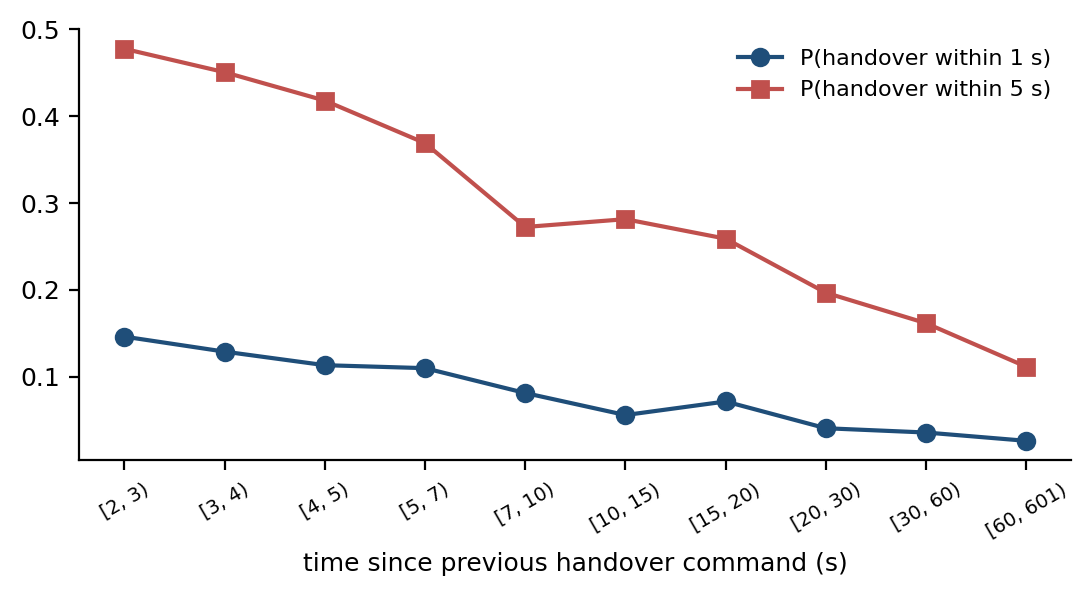
\includegraphics[width=0.80\linewidth]{figures/fig_c8_dwell.png}
\caption{Probability of a handover command within one and five seconds against the time since the previous command. The hazard spikes after a recent handover, reflecting self-excitation.}
\label{fig:5_13}
\end{figure}


\section{The A3 report-conversion rate and the unit it is counted in}
\label{sec:5_9}

The first of the two network characterisations concerns what happens to a measurement report after it is sent, and it is reported here in a corrected form. Event A3 report configurations on this network carry reportInterval and reportAmount values that cause a triggered condition to be re-reported periodically until it ceases: the modal configuration re-reports every 240 ms with reportAmount infinity. Counting transmitted reports therefore counts re-reports of the same trigger, and an earlier draft of this work did exactly that. Table~\ref{tab:5_12} reports the fraction of Event A3 reports that are not followed by a handover command within two seconds across three counting units.


\begin{table}[htbp]
\centering
\caption{Event A3 report conversion, counted per transmitted report and per trigger episode.}
\label{tab:5_12}
\vspace{0.4em}
\singlespacing
\footnotesize
\resizebox{\linewidth}{!}{%
\begin{tabular}{l c c c c}
\toprule
\textbf{Unit} & \textbf{Stratum} & \textbf{n} & \textbf{Followed by a command within 2 s} & \textbf{Declined} \\
\midrule
per report (v1 unit) & pooled & 8,136 & 3006 & 63 \% \\
per report (v1 unit) & 1st Campaign (urban arterial) & 2,287 & 980 & 57 \% \\
per report (v1 unit) & 2nd Campaign (urban loop) & 1,857 & 716 & 61 \% \\
per report (v1 unit) & 3rd Campaign (dense urban) & 2,215 & 806 & 64 \% \\
per report (v1 unit) & 4th Campaign (highway) & 1,777 & 504 & 72 \% \\
per report (v1 unit) & inter-frequency & 93 & 34 & 63 \% \\
per report (v1 unit) & intra-frequency & 8,043 & 2972 & 63 \% \\
per trigger episode (any command within 2 s) & pooled & 2,361 & 1647 & 30 \% \\
per trigger episode (any command within 2 s) & 1st Campaign (urban arterial) & 726 & 531 & 27 \% \\
per trigger episode (any command within 2 s) & 2nd Campaign (urban loop) & 476 & 349 & 27 \% \\
per trigger episode (any command within 2 s) & 3rd Campaign (dense urban) & 740 & 480 & 35 \% \\
per trigger episode (any command within 2 s) & 4th Campaign (highway) & 419 & 287 & 32 \% \\
per trigger episode (any command within 2 s) & inter-frequency & 49 & 28 & 43 \% \\
per trigger episode (any command within 2 s) & intra-frequency & 2,312 & 1619 & 30 \% \\
per trigger episode (one-to-one, owns the command) & pooled & 2,361 & 635 & 73 \% \\
per trigger episode (one-to-one, owns the command) & 1st Campaign (urban arterial) & 726 & 210 & 71 \% \\
per trigger episode (one-to-one, owns the command) & 2nd Campaign (urban loop) & 476 & 110 & 77 \% \\
per trigger episode (one-to-one, owns the command) & 3rd Campaign (dense urban) & 740 & 197 & 73 \% \\
per trigger episode (one-to-one, owns the command) & 4th Campaign (highway) & 419 & 118 & 72 \% \\
per trigger episode (one-to-one, owns the command) & inter-frequency & 49 & 12 & 76 \% \\
per trigger episode (one-to-one, owns the command) & intra-frequency & 2,312 & 623 & 73 \% \\
command multiplicity & A3 episodes & 2,361 & 1647 claimed, 635 owned & x2.59 over-counting \\
command multiplicity & all episodes & 9,819 & 4391 claimed, 908 owned & x4.84 over-counting \\
per trigger episode, by profile & +1 dB, Hys 1, TTT 320, RI 240 x infinity & 734 & 717 claimed, 463 owned & 2.3 \% / 36.9 \% one-to-one \\
per trigger episode, by profile & -15 dB, Hys 1, TTT 160, RI 5120 x infinity & 543 & 274 claimed, 26 owned & 49.5 \% / 95.2 \% one-to-one \\
per trigger episode, by profile & -10 dB, Hys 2, TTT 640, RI 5120 x infinity & 431 & 315 claimed, 71 owned & 26.9 \% / 83.5 \% one-to-one \\
per trigger episode, by profile & -10 dB, Hys 2, TTT 640, RI 5120 x r1 & 278 & 113 claimed, 19 owned & 59.4 \% / 93.2 \% one-to-one \\
per trigger episode, by profile & -15 dB, Hys 1, TTT 160, RI 2048 x infinity & 242 & 141 claimed, 19 owned & 41.7 \% / 92.1 \% one-to-one \\
\bottomrule
\end{tabular}%
}
\end{table}


\begin{figure}[htbp]
\centering
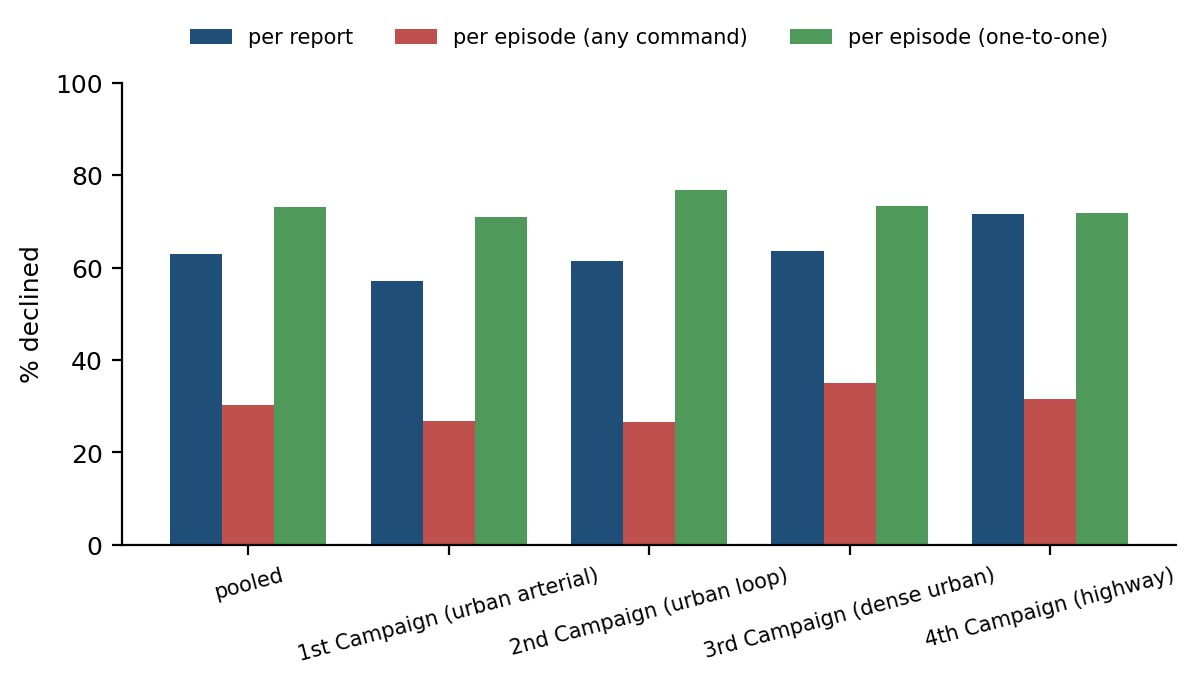
\includegraphics[width=0.80\linewidth]{figures/fig_c7_conversion.png}
\caption{A3 report conversion under three units. Counting transmitted reports counts periodic re-reports, masking the true trigger-episode conversion rate.}
\label{fig:5_14}
\end{figure}

That second figure is not a true conversion rate, and an earlier version of this work reported it as though it were. Several measIds monitor different neighbours and fire within the same approach to a cell boundary, so the 2,361 episodes claim 1,647 commands between them out of the 957 that exist: the same command is claimed by 2.6 episodes on average. Matching each command to exactly one episode containing its most proximate associated report---and resolving the 16 multi-command episodes where rapid consecutive handovers occur---leaves 635 episodes owning commands, so 73\% of episodes are not followed by a matched command. Under loose attribution, a configuration that re-reports on several identities scores a lower unconverted rate precisely because it is verbose, which inverts the interpretation the rate is used for.

The sensitivity to definition is the central finding. A rate quoted without its unit is a statement about counting conventions rather than base-station control policy, and the unconverted share of a mobility trigger moves by a factor of two and a half between two defensible definitions of a single trial. On the command side, 651 of 957 handover commands are temporally associated with an A3 report within two seconds, resolving to 635 unique episodes under one-to-one pairing.

The per-profile breakdown, also in Table~\ref{tab:5_12}, is where the substantive result survives, and it survives more clearly under the stricter unit. The dominant mobility profile---+1 dB offset, 1 dB hysteresis, 320 ms time-to-trigger, 240 ms report interval---is not followed by a command on 36.9\% of its episodes one-to-one, against 95.2\% for the dominant negative-offset configuration. Under the loose unit the same pair reads 2.3\% against 49.5\%: the separation is present either way, and the strict unit widens it, because the negative-offset configurations turn out to be followed by almost no commands at all. That is what characterizes them empirically as neighbour-monitoring rather than mobility triggers.

The conclusion for the literature is therefore not a single conversion percentage. It is that a study using A3 reports as proxy labels for handovers must state its unit, must not let overlapping trigger episodes claim the same command, and must separate the mobility configuration from the rest before drawing conclusions about handover intent.

The finding itself is that a measurement report is not a handover decision. Nearly two thirds of the A3 reports this network receives are declined, and the decline rate rises with cell size. Any model that treats an A3 report as a proxy label for a handover is therefore training on a label that is wrong most of the time.


\section{Ping-pong: definitional instability and its actual source}
\label{sec:5_10}

The rate moves by 17 percentage points --- from 26.3\% to 43.8\% --- without a single change to the underlying measurement. This is the quantitative form of the observation in Section 2.4, and it is why this thesis quotes the strictest of the three and states the alternatives alongside it. It also explains how Amirova et al. \cite{ref15} arrive at 0.13 \% on comparable data: dividing by measurement records rather than by handovers changes the denominator by two orders of magnitude.


\begin{table}[htbp]
\centering
\caption{The ping-pong rate on one fixed set of 957 handover commands under three definitions.}
\label{tab:5_13}
\vspace{0.4em}
\singlespacing
\small
\begin{tabularx}{\linewidth}{X c c}
\toprule
\textbf{Definition} & \textbf{Handovers} & \textbf{Rate} \\
\midrule
Return to the immediately previous cell, identified by PCI and carrier, within 15 s & 957 & 26.3 \% \\
The same, with the cell identified by PCI alone & 957 & 31.2 \% \\
Any return within the window, not only to the previous cell & 957 & 43.8 \% \\
\bottomrule
\end{tabularx}
\end{table}

The window length is a fourth choice, and Figure 5.15 reports the full grid rather than the single row of Table~\ref{tab:5_13}. Across three window lengths and three identity-and-return conventions the same 957 commands yield nine defensible ping-pong rates between 21.0\% and 43.8\%. No cell in that grid is wrong; what is wrong is publishing one of them without saying which.



\begin{figure}[htbp]
\centering

\includegraphics[width=0.85\linewidth]{figures/fig37_pingpong_heatmap.png}
\caption{The ping-pong rate over the full definitional grid: three return windows against three conventions for cell identity and return, computed on one unchanging set of 957 handover commands.}
\label{fig:5_15}
\end{figure}


\begin{table}[htbp]
\centering
\caption{Ping-pong rate by carrier relationship and mobility regime.}
\label{tab:5_14}
\vspace{0.4em}
\singlespacing
\small
\begin{tabularx}{\linewidth}{p{5.5cm} c c c}
\toprule
\textbf{Stratum} & \textbf{Handovers} & \textbf{Ping-pongs} & \textbf{Ping-pong rate} \\
\midrule
intra-frequency handovers & 748 & 233 & 31.1 \% \\
inter-frequency handovers & 209 & 19 & 9.1 \% \\
highway campaign & 177 & 57 & 32.2 \% \\
urban campaigns & 780 & 195 & 25.0 \% \\
all commands & 957 & 252 & 26.3 \% \\
\bottomrule
\end{tabularx}
\end{table}


\begin{figure}[htbp]
\centering
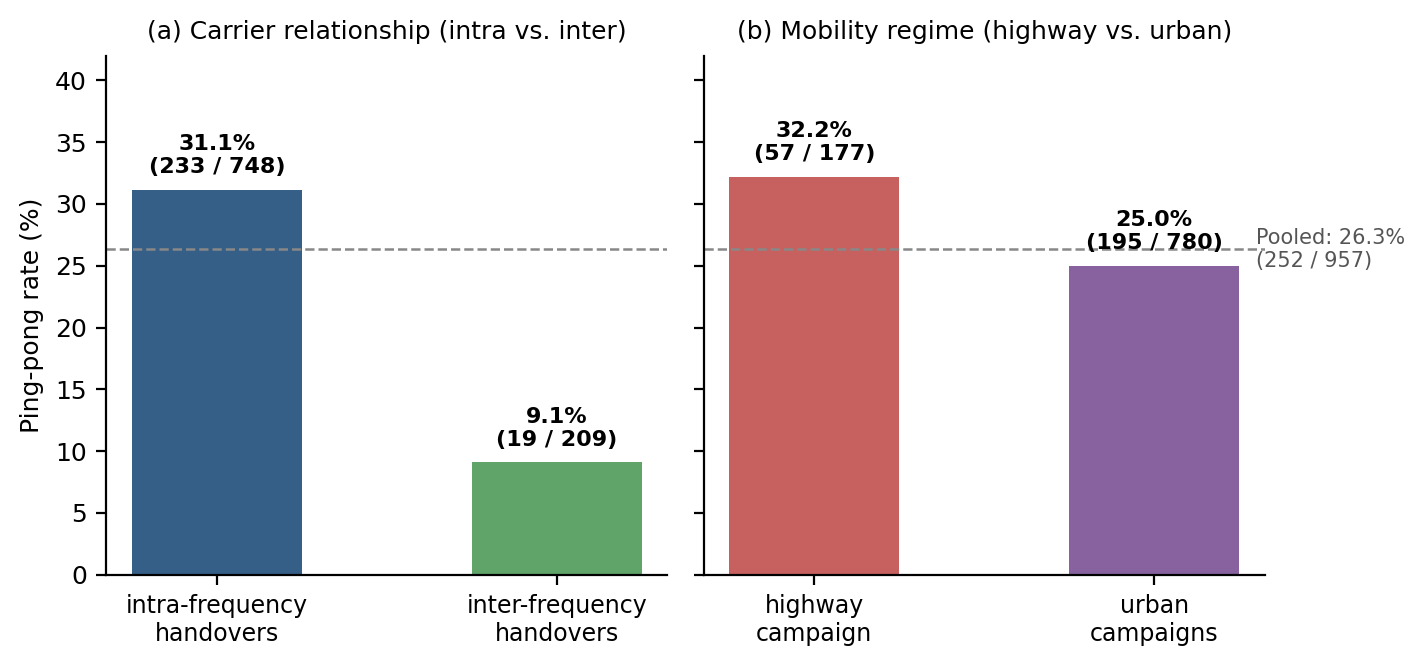
\includegraphics[width=0.88\linewidth]{figures/fig_c13_strata.png}
\caption{Where ping-pong concentrates. The dominant axis is the carrier relationship, not the mobility regime.}
\label{fig:5_16}
\end{figure}

One contrast is large and one is not what it appears to be. Ping-pong concentrates in intra-frequency handovers, at 31.1\% against 9.1\% across carriers, a factor of roughly three: a return to the cell just left is overwhelmingly a return within the same carrier, which is what the A3 entry condition on a single frequency makes easy. The speed contrast points the other way from the intuitive account and cannot be resolved here. The highway campaign, at roughly twice the urban mean speed, returns at 32.2\% against 25.0\% on the urban campaigns --- higher, not lower. With one campaign per regime, speed is completely confounded with route, cell density, carrier mix and time of day, so this thesis does not claim that speed drives ping-pong and does not claim to have ruled it out; it reports that the fastest campaign is also the most return-prone, which is the opposite of what a speed-protective account would predict. Importantly, a rapid return to the previous cell identifies an oscillatory transfer under cellular operational rules, but does not by itself prove that the initial handover was counterfactually unnecessary: without observing link quality had the handset remained on the serving cell (which may have suffered severe fading or link failure), a rapid return reflects sensitive boundary triggering rather than established service degradation.

An earlier version of this section named the time-to-trigger and offset of the dominant configuration profile as the lever available to an operator. That claim is withdrawn. Section 3.5 establishes that the inventory of configuration profiles is static across all four campaigns (with the dominant mobility profile maintaining a fixed offset of +2~dB and time-to-trigger of 320~ms throughout), so neither parameter varies dynamically or across sessions to allow identifying its causal effect on the return rate from these observational measurements at all. The time-to-trigger remains the most plausible lever on theoretical grounds and the obvious candidate for the controlled experiment proposed in Section 7.3, but nothing measured here bears on it.

Modelling the arrival stream as a self-exciting process characterises the clustering from a different direction. The fitted Hawkes branching ratio is 0.653 on the pooled stream, with per-campaign estimates from 0.487 to 0.675. The physical reading of that quantity --- the expected number of direct offspring per event --- belongs to the exponential-kernel model, and the Ogata residual test of Section 4.11 rejects that kernel on this data: rescaling the time axis by the fitted compensator gives 953 residuals whose Kolmogorov--Smirnov distance from a unit-rate exponential is D = 0.065 at p = 0.0007. Their mean is 0.991, indicating that while the average rate is well-matched, the stationary exponential Hawkes model as a whole is rejected by the data. Such a rejection may reflect non-exponential decay dynamics, a time-varying background rate $\mu$(t) driven by corridor transitions and junctions, or unobserved network covariates. The rejection and its statistic are reported rather than suppressed, and together they limit what the number may be used for: the branching ratio is taken here as a comparable summary statistic of how strongly arrivals cluster, not as a count of triggered handovers. The clustering itself is not in doubt, and it is the reason Section 5.8 separates quiet rows from rows inside a burst. Figure 5.17 gives the per-campaign estimates with their intervals and Figure 5.18 illustrates the fitted intensity against the arrival stream itself.


\begin{figure}[htbp]
\centering
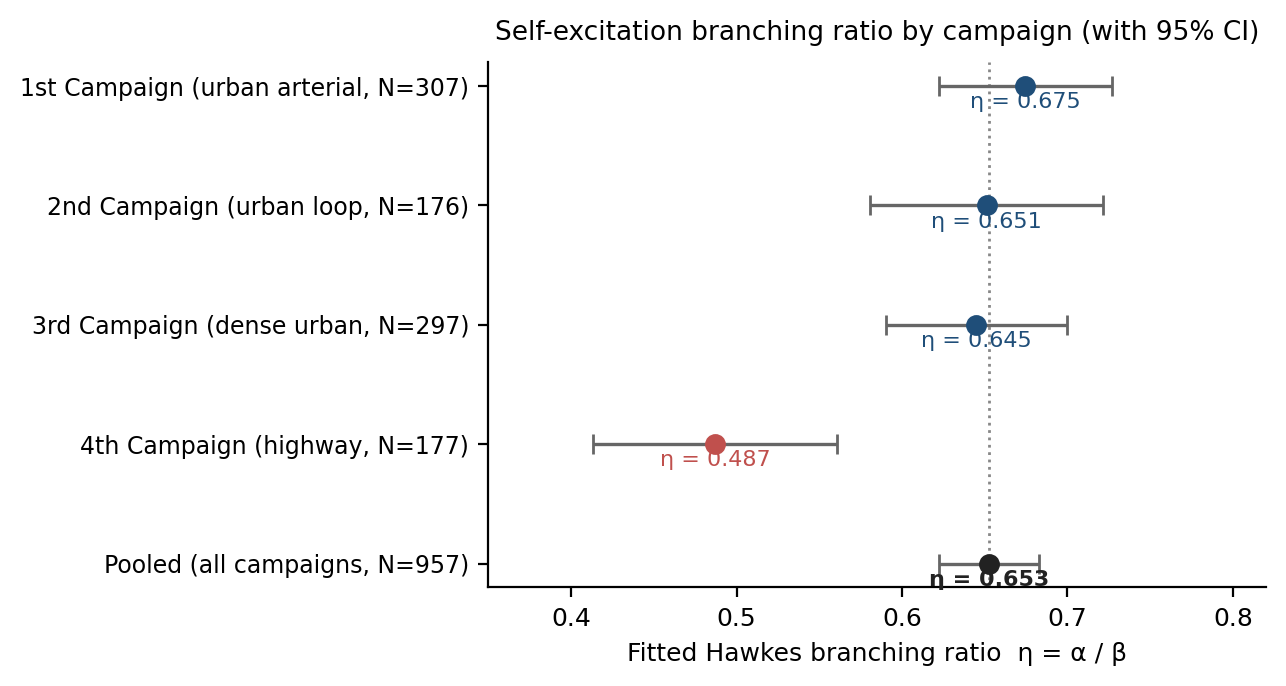
\includegraphics[width=0.80\linewidth]{figures/fig_c_hawkes_branching.png}
\caption{Hawkes branching ratio estimated on each campaign separately and on the pooled stream, with bootstrap confidence intervals. While sub-critical branching ratios indicate substantial empirical clustering ($\hat{\eta} \approx 0.49$--$0.68$), the stationary exponential-kernel model is rejected by Ogata residual testing ($p = 0.0007$), so the ratio is reported as an index of clustering rather than a validated structural generative model.}
\label{fig:5_17}
\end{figure}


\section{Negative results and the cost of the audit}
\label{sec:5_11}

Five approaches were implemented in good faith, measured, and did not help; they are reported because a claim that the formulation and the protocol are what matter is credible only if the alternatives were tried. Table~\ref{tab:5_15} lists them.


\begin{table}[htbp]
\centering
\caption{Approaches implemented and measured that produced no improvement.}
\label{tab:5_15}
\vspace{0.4em}
\singlespacing
\small
\begin{tabularx}{\linewidth}{p{4.0cm} X}
\toprule
\textbf{Approach} & \textbf{Outcome} \\
\midrule
A dedicated ping-pong classifier & AUROC 0.51 at the one-second horizon --- chance \\
Deep CORAL and a second unsupervised domain-adaptation method & No gain over source-only training \\
Sequence models (GRU, TCN, Transformer) on the same features & No gain over gradient-boosted trees; best sequence AUPRC at 1 s 0.167 against 0.179 \\
The signalling feature block added to the main set & AUPRC at 1 s 0.168 against 0.179 without it \\
The unlagged (v1) feature alignment & AUPRC at 1 s 0.600, an artefact of the export row semantics (Section 5.1) \\
\bottomrule
\end{tabularx}
\end{table}


\begin{table}[htbp]
\centering
\caption{Nine cases drawn at random, with a fixed seed, from the out-of-fold predictions at the 5 \% false-positive operating point. Serving RSRP and SINR are synchronous 1~Hz measurements; Gap is computed from held neighbour reports (held under a 3.0~s zero-order hold with median report age $\approx 0.27\text{ s}$). Traces illustrate discrete feature patterns on the sample grid, rather than continuous PHY-layer state machines.}
\label{tab:5_16}
\vspace{0.4em}
\singlespacing
\footnotesize
\resizebox{\linewidth}{!}{%
\begin{tabular}{l c c c c c c c}
\toprule
\textbf{Case} & \textbf{Campaign} & \textbf{Score} & \textbf{To next command (s)} & \textbf{RSRP (dBm)} & \textbf{SINR (dB)} & \textbf{Gap (dB)} & \textbf{Speed (km/h)} \\
\midrule
true positive & 1st Campaign & 0.30 & 0.02 & -80 & -2 & 4 & 40 \\
true positive & 1st Campaign & 0.22 & 0.38 & -101 & -4 & 4 & 72 \\
true positive & 4th Campaign & 0.52 & 0.80 & -108 & 2 & -2 & 76 \\
false alarm & 4th Campaign & 0.60 & 3.85 & -93 & -4 & -4 & 75 \\
false alarm & 4th Campaign & 0.45 & 1.85 & -108 & -16 & -11 & 61 \\
false alarm & 4th Campaign & 0.25 & 34.86 & -114 & -6 & 2 & 80 \\
missed handover & 1st Campaign & 0.08 & 0.82 & -90 & 0 & --- & 45 \\
missed handover & 1st Campaign & 0.07 & 0.21 & -77 & -1 & 3 & 64 \\
missed handover & 3rd Campaign & 0.03 & 0.04 & -80 & -3 & 34 & 41 \\
\bottomrule
\end{tabular}%
}
\end{table}


\begin{figure}[htbp]
\centering
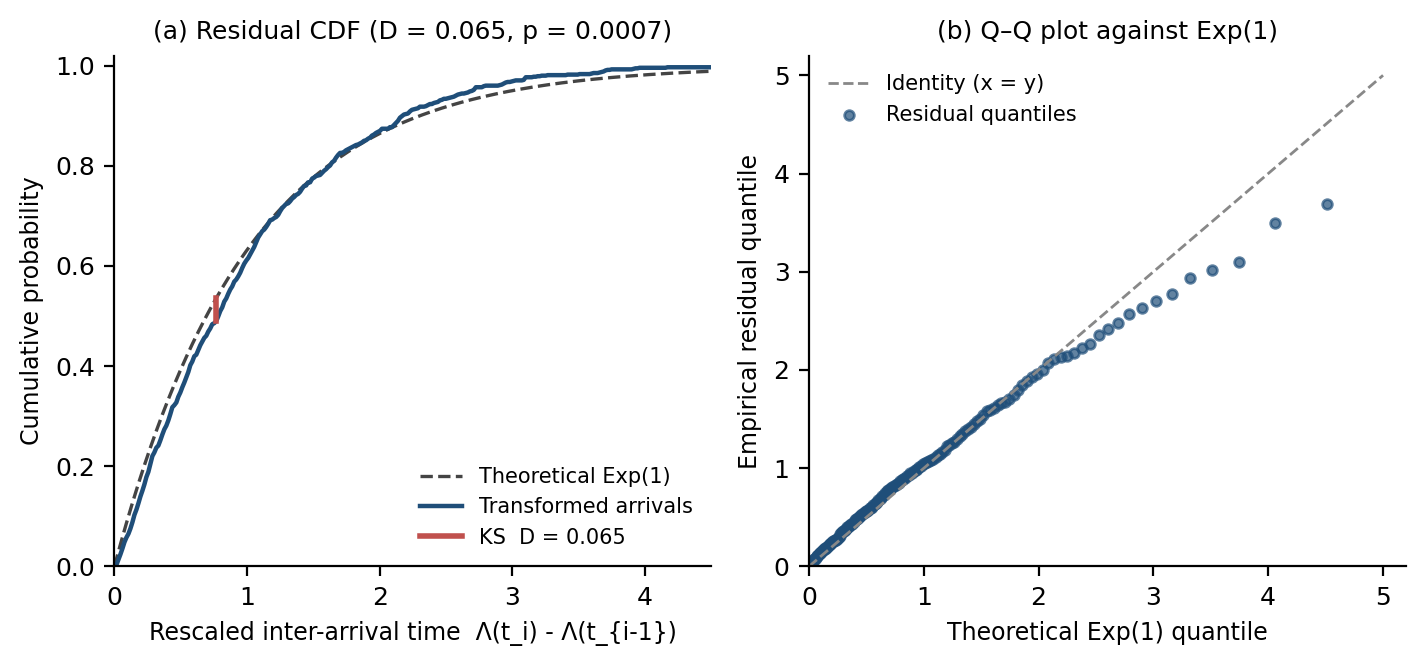
\includegraphics[width=0.88\linewidth]{figures/fig_c_hawkes_residuals.png}
\caption{Self-excitation in the handover arrival stream. While the Ogata residual test formally rejects the stationary exponential kernel ($D = 0.065, p = 0.0007$, likely due to time-varying background rate and corridor transitions), the fitted intensity captures the strong empirical clustering of handovers into bursts.}
\label{fig:5_18}
\end{figure}


\begin{figure}[htbp]
\centering
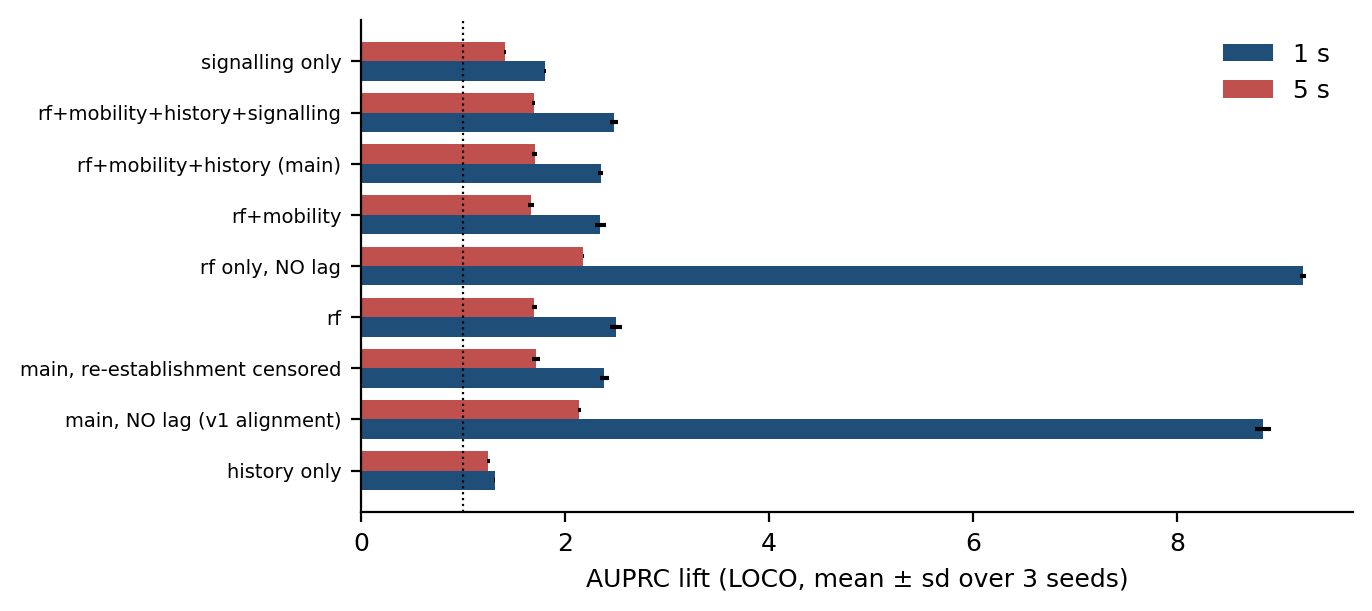
\includegraphics[width=0.88\linewidth]{figures/fig_c18_ablation.png}
\caption{Feature-block, alignment and censoring ablations at one and five seconds, out of fold under leave-one-campaign-out.}
\label{fig:5_19}
\end{figure}

The domain-adaptation null is consistent with published benchmarking rather than indicative of a faulty implementation. Ismail Fawaz et al. \cite{ref27} benchmark nine unsupervised domain-adaptation algorithms over twelve time-series datasets and find several published methods performing worse than source-only training, with the adaptation technique rather than the backbone driving the outcome; the result here has the same shape. The same caution applies to the sequence-model arms: this is a four-session corpus, and the finding is that these architectures do not help on it, not that they cannot help on this task. Recent work is actively developing exactly those architectures for handover prediction on larger corpora \cite{ref45}, \cite{ref46}, and nothing measured here contradicts it.

Aggregate metrics can hide whether a model has learnt something or is exploiting an artefact, and this thesis reported none of the individual cases until a reviewer observed that the only trace it showed anywhere was the idealised schematic of Figure 1.1. Table~\ref{tab:5_16} and Figure 5.20 correct that. Nine rows were drawn uniformly at random, under a fixed seed, from the out-of-fold predictions at the operating point of Section 5.5: three the model scored above threshold with a command following within one second, three it scored above threshold with no command following, and three it scored below threshold with a command following. Nothing was chosen for being illustrative, which is the point of showing them.

Three things are visible in them that no aggregate reports. The first is that real discrete feature traces do not match the idealized continuous trajectory of Figure~1.1: while serving RSRP is refreshed synchronously at 1~Hz, the best-neighbour curve is causally held from event-triggered reports (with a median report age of 0.27~s, bounded by the 3.0~s expiration window). The curves cross repeatedly in the feature matrix, dip several decibels between consecutive seconds, and recross without a handover command being decoded. Importantly, comparing fresh serving RSRP with older, held neighbour measurements reflects an observed feature pattern on the sample grid rather than a verified simultaneous physical A3 entry condition, which requires continuous Layer 3 filtered evaluations at the UE. The second is that false alarms are not arbitrary: in the drawn cases the model alarms where the held neighbour feature temporarily exceeds the serving cell on the grid and no handover command follows within the prediction horizon; these errors reflect transient margin inversions in the feature stream that do not culminate in commands, rather than arbitrary classification noise. Without reconstructing the eNodeB's internal sub-second timer state, one cannot conclude whether the network formally evaluated and declined an entry condition or whether fading transients failed to sustain the required time-to-trigger. The third is that the misses are quiet-looking rows whose command arrives with no visible precursor in the radio trace at all, which is consistent with the modest ceiling reported throughout Chapter 5 rather than with a model that could be repaired by tuning.

These are nine cases and are offered as such. They cannot establish a rate and are not used to; the rates are in Table~\ref{tab:5_3} and Appendix A. What they establish is that the model's errors have a structure a reader can inspect, which is a claim that could not be checked at all before they were shown.

The largest negative result in this thesis is the alignment audit of Section 5.1, and it is recorded here as such: the strongest configuration this project measured --- AUPRC 0.600 at one second --- was an artefact of a one-second misalignment between the measurement grid and the event clock, and the corrected figure is 0.179. Retaining that result would have produced a more impressive thesis and a false one.

As recorded in Table~\ref{tab:5_15}, adding the ten explicit control-plane state features (A3 report counts, hold times, and deployed thresholds) to the main feature set changes the one-second AUPRC from 0.179 to 0.168, confirming that the primary radio, mobility and session-history features already capture the available imminence information, and that incorporating active control-plane state confers no additional predictive lift.


\begin{figure}[htbp]
\centering
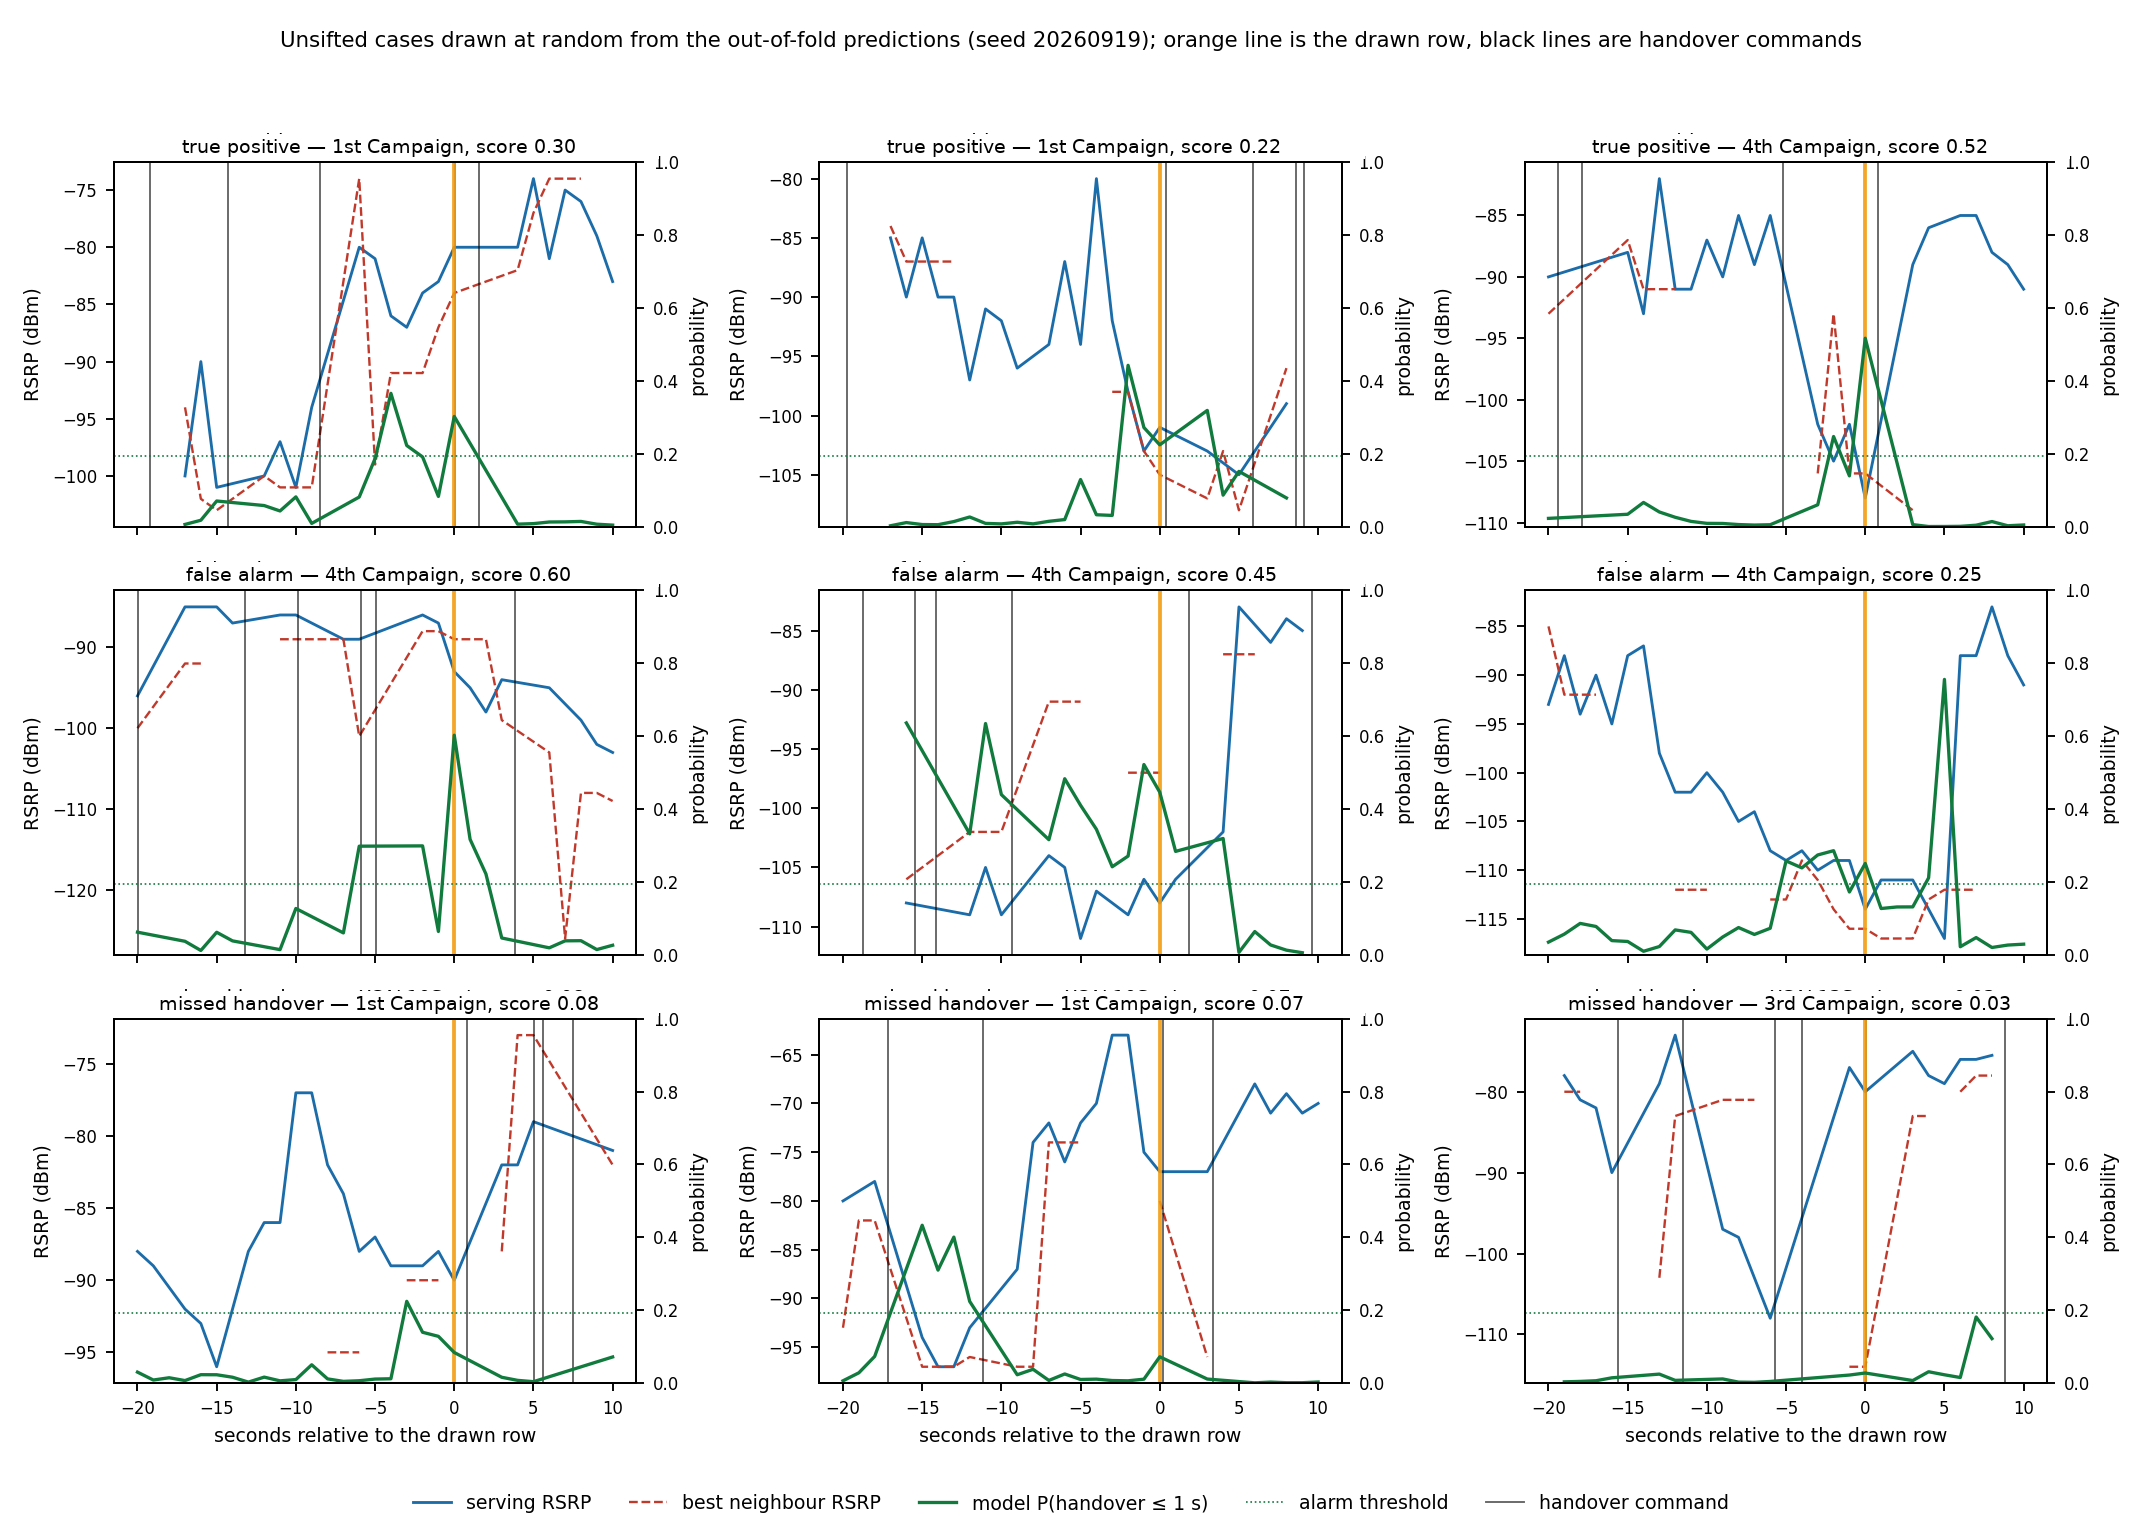
\includegraphics[width=0.95\linewidth]{figures/fig_c20_cases.png}
\caption{Nine cases drawn uniformly at random, with a fixed seed, from the out-of-fold predictions at the 5 \% false-positive operating point. Blue: serving RSRP (1~Hz export); Red: best neighbour RSRP (zero-order hold from decoded reports, with median observation age $\approx 0.27\text{ s}$); Green: model probability of command within 1 s. Traces reflect observed feature patterns rather than continuous internal PHY/RRC state machines.}
\label{fig:5_20}
\end{figure}

Finally, removing the signalling leakage guard of Section 4.6 raises the apparent score substantially, which is the expected behaviour of a leak and is the reason the guard exists. That configuration is not reported as a result anywhere in this thesis.


\section{Discussion against the objectives}
\label{sec:5_12}

Objective O1 is met in a qualified form: the next handover command is predicted within the next second (horizon $h_1 = 1\text{ s}$, with an empirical median lead time $\approx 0.47\text{ s}$) at AUPRC 0.179 against a 6.8\% floor (2.6x) and AUROC 0.777, from quantities a handset observes strictly before the prediction instant, against AUPRC 0.116 for the implemented A3 signal-margin proxy. The qualification is that this is a modest signal, well short of what an uncorrected protocol reports on the same data.

Objective O2 is met, and the answer is larger than the modelling differences the thesis reports. Between the leakiest and the soundest protocol the one-second AUPRC of the primary model moves by 48 \%, and a one-row misalignment moves it by 236 \% --- both larger than the gap between the best and worst learner under a fixed protocol.

Objective O3 is met in part. Coherence is exact by construction, and the conformal formulation is reported with the alarm rate it costs, the feasibility floor set by the number of calibration units, and the measured behaviour in the non-exchangeable regime. The part that is not met is the estimand: the bound evaluated here is over rows, and the per-handover bound the objective asks for cannot be certified at one second on a one-hertz grid at all, because 36.4\% of commands have no usable row in their lead window under the post-handover blanking policy. It becomes expressible at three seconds, at an alarm rate near one second in two. The second part that is not met is exchangeability itself: calibrating on one campaign and evaluating on another represents the cross-environment deployment regime. The empirical mean miss loss across held-out campaigns was 0.153 at a target of $\alpha = 0.20$. However, cross-campaign results cannot be certified as formal distribution-free guarantees because macro-environmental shifts violate exchangeability, and the 12 pairwise campaign rotations exhibit pseudoreplication across $n=4$ physical sessions. Both limitations are properties of the operational setting rather than of the procedure, and the objective is reported as partly met on that basis rather than restated to fit what was achieved.

Objective O4 is partially met with structural confounding: leave-one-campaign-out achieves AUROC between 0.765 and 0.805 across held-out sessions, including 0.769 on the highway corridor. However, vehicle speed and corridor geography are structurally collinear on Campaign 4, preventing unique attribution of the performance gap, and Campaign 4 was evaluated in retrospective diagnostic exploration of the alignment repair. Furthermore, cross-corpus transfer achieves AUROC 0.760 on an external public dataset from the same operator and metropolitan area [38], but this transfer is evaluated on common L3 signalling features rather than the complete 112-feature multi-modal model due to schema limitations in the public release.

Objective O5 is met in corrected form. The single strongest lesson is methodological --- the alignment audit --- and the substantive one is that the quantity Event A3 thresholds on is a weak predictor of imminence (AUROC 0.618 alone), while no single available feature replaces it.


\section{Threats to validity}
\label{sec:5_13}

The methodological and empirical findings of this thesis are subject to threats across four standard dimensions of validity, which are explicitly addressed below.

\subsection{Internal validity}
Internal validity concerns whether the observed relationships between features, protocols, and event occurrences are genuine rather than artefacts of measurement or preprocessing.
\begin{itemize}
    \item \textbf{Export timestamp alignment and feature ageing:} As documented in Section~\ref{sec:5_1}, periodic 1~Hz logging exports exhibit end-of-second aggregation semantics, corrupting pre-handover rows with post-handover serving-cell identities in 76\% of cases. Applying a one-row lag completely eliminates this look-ahead contamination, but inevitably introduces one second of information ageing across uncorrupted radio and kinematic features. The 211 residual cases where $m > 0$ yet row $t$ shows the source cell reflect an exporter refresh buffer delay rather than a failure of the aggregation model, as verified in Table~\ref{tab:A_6}.
    \item \textbf{Residual burst contamination at row $t-1$:} Row $t-1$ shows the target cell in 11.7\% of isolated handovers and 15.6\% of all handovers. In both subsets this is below the subset's own earlier rows (12.1\%/12.1\% and 21.7\%/23.7\% at rows $t-2$/$t-3$), so there is no step at row $t-1$; the higher pooled level reflects ping-pong returns to recently serving cells. Model lift is also highest on quiet rows (3.1$\times$ vs 1.9$\times$ in bursts; Section~\ref{sec:5_8}, Table~\ref{tab:5_11}), which is inconsistent with residual burst contamination driving the result.
    \item \textbf{Protocol design leakage on Campaign 4:} Although Campaign 4 was held out during model parameter estimation and hyperparameter selection, it was examined during retrospective diagnostic exploration of the timestamp alignment defect; hence Campaign 4 is an out-of-sample test unit for learned model weights, but not a blind prospective holdout for pipeline feature engineering.
    \item \textbf{Preprocessing and blanking window policy:} To prevent post-handover transient states from contaminating consecutive predictions, an operational 2~s blanking window is enforced following each handover command. While necessary to avoid predicting trivial immediate successors, this policy mechanically sets the maximum achievable fraction of resolvable handovers at 64.2\% at the 1~s horizon (leaving 35.8\% unresolvable in continuous driving, rising to 36.4\% under chunk boundary cuts).
    \item \textbf{Post-hoc parameter thresholds and repository freeze:} The 180~s block duration, 60~s temporal purge, 10~s burst cutoff, and 2~s blanking window were selected during protocol design. Although frozen in the internal project version control repository prior to Campaign 4 acquisition, this internal freeze was not registered with an independent external trial registry. Sensitivity analysis across parameter ladders (Table~\ref{tab:A_5}) confirms local numerical stability around chosen values.
\end{itemize}

\subsection{External validity}
External validity concerns the generalisability of these findings beyond the specific measurement corpus.
\begin{itemize}
    \item \textbf{Instrumentation and single-device limits:} All four campaigns were recorded using a single commercial drive-test handset model and a single Accuver XCAL diagnostic firmware build. While external cross-instrument replication on NUWiNS confirms that end-of-second export aggregation is an inherent property of XCAL periodic exports, handset-specific baseband firmware logging or diagnostic buffer commit latencies cannot be conclusively separated from network effects without multi-device, multi-firmware replication.
    \item \textbf{Carrier and operator coverage:} All captures were conducted on a single commercial LTE operator in Dhaka and Gazipur. While the deployed Event A3 parameters reflect standard 3GPP configurations (+1~dB offset, 320~ms TTT), handover dynamics under different carrier frequency plans, heterogeneous small-cell deployments, or alternative vendor equipment may alter absolute performance levels.
    \item \textbf{Speed and corridor confounding:} In Campaign 4, vehicle velocity (50.9~km/h vs 21.4--39.1~km/h) and corridor topography (suburban highway vs dense urban corridors) are collinear. The performance variation observed in Section~\ref{sec:5_6} cannot be uniquely separated into velocity-induced Doppler fading versus spatial base-station layout.
    \item \textbf{Schema limits in external transfer and departmental lineage:} External validation on the Shafi et al. \cite{ref38} dataset was restricted to the 6-feature L3 signalling block because the public release lacked synchronous 1~Hz radio metrics and GPS coordinates. Furthermore, that dataset was collected in the same metropolitan area on the same operator by an earlier research cohort in our department; transferability of the complete 112-feature multi-modal model to distinct operators and international markets remains to be established.
\end{itemize}

\subsection{Construct validity}
Construct validity assesses whether the operationalized variables accurately reflect the underlying theoretical constructs.
\begin{itemize}
    \item \textbf{Signal-margin baseline vs.\ internal eNodeB state:} The implemented Event A3 baseline evaluates the radio margin condition $(M_n - M_s > \text{Off} + \text{Hys})$ on the discrete 1~Hz export grid. It serves as an empirical signal-margin proxy rather than an exact emulation of the base station's continuous internal time-to-trigger timer.
    \item \textbf{Signalling commands vs.\ handover necessity:} Ground truth labels are derived from decoded \texttt{RRCConnectionReconfiguration} commands with confirmed completions. While this verifies that a physical handover took place, observational traces cannot establish counterfactual necessity---whether retaining the serving cell would have caused radio link failure or whether the handover was suboptimal.
\end{itemize}

\subsection{Statistical conclusion validity}
Statistical conclusion validity concerns the appropriateness of the statistical methods and sample sizes used to draw inferences.
\begin{itemize}
    \item \textbf{Limited degrees of freedom ($n=4$):} With four continuous drive campaigns, two-sided non-parametric sign tests are bounded by $p \ge 0.125$. Accordingly, all cross-campaign comparisons are reported as empirical effect sizes, spreads, and paired differences rather than claiming null-hypothesis rejection.
    \item \textbf{Temporal autocorrelation and block bootstrap intervals:} While 180~s block bootstrapping provides a descriptive measure of variance, contiguous blocks within the same drive share macro-environmental conditions. Consequently, within-session bootstrap intervals are anti-conservative, and true between-session uncertainty is represented by the LOCO spread [0.132, 0.233].
    \item \textbf{Finite-sample floors in conformal risk control:} Conformal risk control requires $n \ge 1/\alpha - 1$ calibration units to achieve non-trivial threshold selection. For small campaigns ($n \le 20$), tight targets ($\alpha \le 0.05$) mathematically exceed this feasibility floor, defaulting to constant alarm fallback. Furthermore, the 12 pairwise cross-campaign rotations exhibit pseudoreplication ($n=4$ degrees of freedom) and violate exchangeability, rendering cross-campaign risk bounds descriptive diagnostics rather than certified operational guarantees.
    \item \textbf{Multiplicity control:} Model leaderboard comparisons among the seven learners are treated descriptively without multiplicity adjustment, as differences fall within bootstrap confidence intervals. Conversely, formal hypothesis testing on point-process residual goodness-of-fit (Section~\ref{sec:5_10}) strictly enforces Holm--Bonferroni correction across the four campaigns.
\end{itemize}

